\documentclass[12pt,a4paper]{article}
\usepackage[utf8]{inputenc}
\usepackage[lmargin=0.8in, rmargin=0.8in, tmargin=1in, bmargin=1in]{geometry}
\usepackage{setspace}
\usepackage{titling}
\usepackage{lipsum}
\usepackage{comment}
\usepackage{physics}

\usepackage{tikz}
\usetikzlibrary{shapes}
\usetikzlibrary{matrix}
\usepackage[normalsize]{subfigure}
\usetikzlibrary{backgrounds,automata}
\usepackage[
singlelinecheck=false 
]{caption}
\usepackage{float}

\usepackage{amsmath,amsfonts,amssymb,bbm}
\usepackage{mathrsfs} 
\newcommand\numberthis{\addtocounter{equation}{1}\tag{\theequation}}

\usepackage{mathtools, nccmath}
\usepackage[english]{babel}
\usepackage{blindtext}

\usepackage{amsthm} %% the environment for the "proof" format

\newtheorem{prop}{Theorem}
\newtheorem{coro}{Corollary}[prop]

%% citation formatting %%
\usepackage{natbib}
\bibliographystyle{asr}
\setcitestyle{authoryear,open={(},close={)}}
%% end %%

\usepackage{graphicx}
\newcommand{\indep}{\rotatebox[origin=c]{90}{$\models$}}  % the independence symbol

\newcommand{\Cov}{\operatorname{Cov}}
\newcommand{\Var}{\operatorname{Var}}
\newcommand{\E}{\operatorname{E}}

\newcommand{\ATE}{\text{ATE}}
\newcommand{\ATT}{\text{ATT}}

\def\X{{\boldsymbol X}}
\def\x{{\boldsymbol x}}
\def\Q{{\boldsymbol Q}}
\def\q{{\boldsymbol q}}
\def\Z{{\boldsymbol Z}}
\def\z{{\boldsymbol z}}
\newcommand{\A}{\mathrm{A}}
\DeclareMathOperator{\Pro}{Pr}
\def\one{\mathbbm{1}}
\def\P{\mathbbm{P}}
\newcommand{\defeq}{\vcentcolon=}

\def\pheight{\frac{w(\X,\Q,g')}{\E_{\mathcal{P}_t}(w(\X,\Q,g') \mid \Q,g')}}

\usepackage{changepage}  % enables changing page margin for a specific part of the text

\usepackage[colorlinks=true, allcolors=blue, hyperfootnotes=false]{hyperref}  % hyperlinks. And I turned off hyperlinks to footnotes. 

\usepackage{makecell}
\renewcommand{\cellalign}{tl}  % change the vertical and horizontal alignments within "makecell".

\setlength{\parskip}{1em}
\allowdisplaybreaks

\setlength{\tabcolsep}{0.4em}  % change spacing between table columns

%%%%%%%% below is for making appropriately-looking hyperlinks to citations %%%%%%%
\usepackage{etoolbox}
\makeatletter

\pretocmd{\NAT@citex}{%
  \let\NAT@hyper@\NAT@hyper@citex
  \def\NAT@postnote{#2}%
  \setcounter{NAT@total@cites}{0}%
  \setcounter{NAT@count@cites}{0}%
  \forcsvlist{\stepcounter{NAT@total@cites}\@gobble}{#3}}{}{}
\newcounter{NAT@total@cites}
\newcounter{NAT@count@cites}
\def\NAT@postnote{}

% include postnote and \citet closing bracket in hyperlink
\def\NAT@hyper@citex#1{%
  \stepcounter{NAT@count@cites}%
  \hyper@natlinkstart{\@citeb\@extra@b@citeb}#1%
  \ifnumequal{\value{NAT@count@cites}}{\value{NAT@total@cites}}
    {\ifNAT@swa\else\if*\NAT@postnote*\else%
     \NAT@cmt\NAT@postnote\global\def\NAT@postnote{}\fi\fi}{}%
  \ifNAT@swa\else\if\relax\NAT@date\relax
  \else\NAT@@close\global\let\NAT@nm\@empty\fi\fi% avoid compact citations
  \hyper@natlinkend}
\renewcommand\hyper@natlinkbreak[2]{#1}

% avoid extraneous postnotes, closing brackets
\patchcmd{\NAT@citex}
  {\ifNAT@swa\else\if*#2*\else\NAT@cmt#2\fi
   \if\relax\NAT@date\relax\else\NAT@@close\fi\fi}{}{}{}
\patchcmd{\NAT@citex}
  {\if\relax\NAT@date\relax\NAT@def@citea\else\NAT@def@citea@close\fi}
  {\if\relax\NAT@date\relax\NAT@def@citea\else\NAT@def@citea@space\fi}{}{}

\makeatother
%%%%%%%% end %%%%%%%


\linespread{1.6}  % double spacing 
\setlength{\parskip}{0em}  % no paragraph spacing

\title{\Large Nonparametric Causal Decomposition of Group Disparities \thanks{We thank Paul Bauer, Eric Grodsky, Aleksei Opacic, Guanghui Pan, Chan Park, Ben Rosche, and Jiwei Zhao for helpful comments and suggestions. Earlier versions of this paper has been presented at Causality in the Social Sciences Workshop at GESIS in 2021, Population Association of America annual meeting in 2022, and American Causal Inference Conference in 2022. We thank participants at these conferences for constructive discussions, especially our discussant at the first two conferences, Xiang Zhou.}} 

\author{\large Ang Yu\thanks{Department of Sociology, University of Wisconsin-Madison. Email: ayu33@wisc.edu} \and Felix Elwert\thanks{Department of Sociology and Department of Biostatistics and Medical Informatics, University of Wisconsin-Madison}}
\date{\large \today}

\setstretch{1.5}

\begin{document}

\maketitle

\begin{abstract}
We propose a nonparametric method for decomposing group disparities in terms of an intermediate treatment variable. Our decomposition contains four components capturing the contributions of group differences in baseline characteristics, treatment prevalence, average treatment effect, and selection into treatment. These components readily inform policy interventions on the treatment and its effect. Our main contribution is to neatly separate the roles of between-group and within-group effect heterogeneity in explaining group disparities, revealing a new lever for reducing disparities. This decomposition reformulates the classic Kitagawa-Blinder-Oaxaca decomposition in causal and model-free terms, supplements causal mediation analysis by targeting group disparities instead of group effects, and resolves conceptual difficulties of recent random equalization decompositions. We also provide a conditional decomposition that allows researchers to incorporates pre-treatment covariates in defining the estimand and potential interventions. Using efficient influence functions and cross-fitting, we propose nonparametric estimators that are $\sqrt{n}$-consistent, asymptotically normal, semiparametrically efficient, and doubly robust. We apply our framework to study the causal role of education in intergenerational income mobility. 
\end{abstract}
%%% AOAS and JASA requirement: abstract less than 200 words

\section{Introduction}

Improving the explanations of inter-group disparities is an urgent task for the social and health sciences. For example, what is the contribution of educational attainment to racial disparities in adult health? How much of the gender wage gap can be explained by occupational sorting? And what is the role of college completion in the relationship between parental income and income during adulthood? 
The structure of such question is always the same. Researchers compare the outcomes of two groups whose membership is typically established early in life (e.g., race, gender, parental background, birth cohort, country) and ask how differences in outcomes can be attributed to some intermediate treatment variable that occurs between the establishment of group membership and the outcome. 

Questions about explanations, contributions, and attribution \citep[e.g.,][]{morgan_models_2012,barber_black-white_2015,mize_sexual_2016,brady_rethinking_2017, bernardi_compensatory_2020,storer_what_2020,zajacova_pain_2021} are inherently causal. First, researchers often are interested in the \emph{causes} of disparities and ask counterfactual questions about the impact of changing one or more intermediate variables, which is necessary for informing real-world interventions that could alleviate the disparities. It is one thing to observe that racial differences in college completion coexist with wage gaps by college completion status; it is another to establish that differences in college completion are responsible for racial wages gaps, such that intervening to equalize college graduation rates would remediate wage inequality. Second, researchers often also posit counterfactual scenarios where the effects of an intermediate variable in a group were set to different values than they are in reality. At a minimum, the discussion of effects also presumes causal identification. 

Three prior approaches are concerned with questions of attribution and explanation.  
First, the Kitagawa-Blinder-Oaxaca (KBO) decomposition \citep{kitagawa_components_1955, blinder_wage_1973, oaxaca_male-female_1973} is a classic tool used for explaining group disparities and remains popular to this day \citep[e.g.,][]{barber_black-white_2015, mize_sexual_2016,laurison_class_2016, storer_what_2020, zajacova_pain_2021}. The KBO decomposition is based on group-specific linear regression models and decomposes the group disparity into an explained component and an unexplained component. The explained component reflects the differential averages of an intermediate variable by group, and the unexplained component captures differential slopes and intercepts. The classic KBO decomposition is thus defined in terms of regression coefficients and not nonparametrically formulated in causal terms. This renders the KBO decomposition inappropriate for explanation and attribution question. In fact, sociologists and economists alike have criticized the KBO decomposition for failing to answer any  counterfactual question by design (\citeauthor{fortin_decomposition_2011}, \citeyear{fortin_decomposition_2011}, p.13; \citeauthor{lundberg_what_2021}, \citeyear{lundberg_what_2021}, p.542). 

Second, causal mediation analysis is also used to attribute the relationship between two variables to an intermediate variable \citep{vanderweele_explanation_2015}. Causal mediation estimands are clearly defined in counterfactual terms, however, they are not designed for explaining group disparities. This is because what they decompose are summary measures of treatment effects, such as the Average Treatment Effect (ATE). However, the discussion of treatment effects is conceptually challenging when it comes to ascriptive variables such as race and gender, as it is not plausible to impose any intervention on these variables. Some group variables, such as early-life socioeconomic status, can theoretically be intervened upon, but not for people who are already later in their life course. Indeed, in numerous applications in social and health sciences, descriptive group disparities, rather than an effect, is what researchers seek to understand and explain. Causal attribution of group disparities thereby requires analytical frameworks more tailored to it than mediation analysis.  

Third, more recently, epidemiologists have developed a causal decomposition of group disparities, which we call the random equalization decomposition \citep{vanderweele_causal_2014, jackson_decomposition_2018}. For this estimand, the extent to which the group disparity can be attributed to the differential prevalence of an intermediate variable is defined as the reduction in disparity brought about by a hypothetical intervention that randomly gives members of the disadvantaged group values of the intermediate variable according to the distribution of the advantaged group. The random equalization decomposition marks a important advancement towards establishing an appropriate framework for causal attribution of group disparities to an intermediate treatment variable. However, as we will show, the random equalization decomposition does not purely capture the contribution of differential prevalence of the intermediate variable. Instead, it also incorporates the influence of differential patterns of selection into treatment across groups, which complicates its interpretation.

In this article, we develop a novel decomposition method for group disparities in terms of an intermediate treatment variable. Our decomposition is defined counterfactually with respect to the treatment variable and descriptively with respect to the group variable. This approach is consistent with common practices in the social sciences and focuses on more modifiable factors in terms of policy intervention. Our decomposition contains four components, respectively capturing the contributions of baseline differences unrelated to the treatment, differential treatment prevalence, differential ATE, and differential selection into the treatment. Compared with the KBO decomposition, our decomposition enables causal attribution and nonparametric estimation. It supplements causal mediation analysis by focusing on explaining group disparities instead of ``effects'' of the group variables. It also improves on the random equalization decomposition by providing components with unambiguous interpretations. The component in our decomposition that captures differential selection is a centerpiece in our contributions. First, this component reveals a novel policy lever for reducing disparities, and it did not appear in any of the previous decompositions. Second, by separating it from the component representing differential prevalence, we clarify the random equalization decomposition and provide a more clearly interpretable decomposition. 

Our paper proceeds as follows. Section 2 formally introduces our decomposition and interventional interpretations. We also formally relate our decomposition to the classic KBO decomposition, a specific causal mediation estimand, and the random equalization decomposition, through which we explicate the contributions of our framework. We also extend the decomposition to a conditional version, which allows researchers to take pre-treatment covariates into account in defining the estimand and potential interventions. In section 3, under the conditional igorability assumption, we develop nonparametric estimators for the unconditional and conditional decompositions based on their efficient influence functions. These estimators can be implemented via data-adaptive methods such as ML and accommodate high-dimensional confounders. We also derive conditions under which the estimators are $\sqrt{n}$-consistent, asymptotically normal, and semiparametrically efficient. In addition, they have double-robustness properties. In section 4, we apply our decompositions to study the causal role of college graduation in intergenerational income mobility. Section 5 concludes with possible extensions. 

%[This para someplace] Intervening variables can ``contribute" to disparities in multiple ways. Prior to determining the value of the exposure, the groups may or may not already experience baseline disparities. Next, one can ask to what extent differences in the effect of the exposure on members of the two groups contribute to outcome disparities; how differences in the prevalence of the exposure in the two groups.... ; and to what extent it matters which members of each group are selected to receive the exposure.  
    %[OR:] Exposures can `contribute' to outcome disparities in several different ways. It matters how many members of each group receive the treatment, which members of each group receive the treatment, and what the effect of the treatment is on the outcome. 
    %[OR:] Exposure can `contribute' to outcome disparities in three different ways. What share of each group receives the exposure? How does the effect of the exposure on the outcome differ between groups on average? And, to the extent that the effect of the exposure varies across individuals within groups, which members of each group receive the treatment?

%When asking about the ‘contribution’ of a variable to an ‘explanation’ of disparities, one needs to define contribution and explanation. Following a long tradition in sociology-reaching back to Weber—we believe that explanations call for a causal account. Contribution…  

\section{The estimand}
\subsection{Unconditional decomposition}
For each individual $i$, consider a binary treatment variable $D_i \in \left\lbrace 0,1 \right\rbrace$. Let $Y_{i0}$ and $Y_{i1}$ be the potential outcomes \citep{rubin_estimating_1974} of $Y_i$ under the hypothetical intervention to set $D_i=0$ and $D_i=1$, respectively. Let $\tau_i \coloneqq Y_{i1} - Y_{i0}$ denote the individual-level treatment effect. Henceforth, we largely suppress individual level subscripts on all variables to unburden notation. Suppose that the population contains two disjoint groups, $g \in \left\lbrace a,b \right\rbrace$, where $a$ denotes the advantaged group and $b$ denotes the disadvantaged group. We use subscripts $g$ to indicate group-specific quantities, for example, $\E_g(Y) \coloneqq \E(Y \mid G=g)$.  

We now only assume SUTVA, i.e.,
\begin{itemize}
     \item[] (A.1) $Y=D Y_1 + (1-D) Y_0$,
\end{itemize}
so that the observed outcome equals the potential outcome under the treatment that was actually assigned.
Then, the observed outcomes disparity between group $a$ and $b$ can be decomposed into four components: 
\begin{align}
&\phantom{{}={}} \E_a(Y)-\E_b(Y)   \nonumber  \\
&= \underbrace{ \E_a(Y_{0})-\E_b(Y_{0}) }_{\text{\normalsize baseline}}
+ \underbrace{\E_b(\tau) [\E_a(D)-\E_b(D)]}_{\text{\normalsize prevalence}} \nonumber  \\ 
&\phantom{{}={}} + \underbrace{\E_a(D)[ \E_a(\tau) - \E_b(\tau) ]}_{\text{\normalsize effect}} 
+ \underbrace{\Cov_a(D, \tau) -  \Cov_b(D, \tau)}_{\text{\normalsize  selection}}. \label{eqt1}
\end{align}
The ``baseline" component reflects the difference in average baseline potential outcome $Y_0$ between groups, i.e., the difference in outcomes if nobody received treatment. The ``prevalence" component indicates how much of the group disparity is due to differential prevalence of treatment. The ``effect" component reflects unequal average treatment effects (ATE) across groups. Finally, the ``selection" component captures the contribution of the differential selection into treatment based on the treatment effect, $\tau$,  to the group disparity. 
For each group, if group members who would gain more from treatment are more likely to receive the treatment than those who would gain less, there will be a positive covariance between $D$ and $\tau$. To our knowledge, none of prior decompositions of group disparities includes a selection component. \footnote{\citet{zhou_attendance_2022} recently developed a causal decomposition method for a special case of mediation analysis, which contains a similar covariance component capturing selection into a mediator.} 
Both the effect and the selection components account for the relationship between heterogeneous effects and group disparities. But the ``effect" component captures the contribution of \emph{between}-group effect heterogeneity; and the ``selection" component captures the contribution of \emph{within}-group effect heterogeneity. In summary, a group will be more advantaged in the outcome if its members have a higher average baseline potential outcome, a higher prevalence of treatment (given a positive ATE), a higher ATE, or a higher level of selection into treatment based on treatment effect.

Our decomposition is formulated in counterfactual terms, hence is prescriptive for future interventions. The decomposition reveals three levers by which a policy may affect inter-group disparities through the treatment. First, policy makers could manipulate the prevalence of the treatment in each of the two groups. Second, they could manipulate who within each group receives treatment. For example, they could facilitate the matching of high-return individuals to treatment receipt in the disadvantaged group. Third, they might even be able to manipulate the effect of exposure on each individual. \footnote{It is more unconventional to discuss interventions on treatment effects than on treatments. However, interventions on effects have appeared in both methodological \citep{malinsky_intervening_2018} and empirical \citep{brady_rethinking_2017} literatures.
Our notion of interventions on effects is a generalization of Malinsky's (\citeyear{malinsky_intervening_2018}) interventions on ``structural features'', as we allow for heterogeneous effects.} Specifically, each of our decomposition component quantifies the part of the outcome disparity that could be eliminated if the two groups were equalized with respect to that component while other characteristics were held unchanged.

To further fix ideas, we may more exactly pin down the equalization intervention implicated by each decomposition component. The prevalence component indicates the part of the disparity that would be eliminated by giving group $b$ the treatment prevalence of group $a$, which can be seen by replacing $\E_b(D)$ with $\E_a(D)$ in equation (\ref{eqt1}). In the same vein, the effect component is the part of the disparity that would disappear if group $a$ was given the ATE of group $b$. Finally, the disparity would be reduced by the amount of the selection component if the two groups were made to have the same selection level, regardless of the specific level at which their selection would be fixed. However, given that the prevalence, effect, and selection components are determined only by two variables, the treatment and the treatment effect, it is not always possible to intervene on a single component without changing the values of other components. Nevertheless, we may alternatively conceive of a whole-package intervention. A whole-package intervention transfers the joint distribution of $D$ and $\tau$ from one group to the other. Our prevalence, effect, and selection components then add to the reduction in disparity of the whole-package intervention, and each of them can be interpreted as a substantive aspect of the intervention.

Using the randomized intervention notation proposed by Didelez et al. (\citeyear{didelez_direct_2006}), there is another way to interpret the decomposition components from an interventional perspective. Extended versions of the randomized intervention notation have been used to define randomized interventional mediation estimands and random equalization decompositions, which we address later. 
Under the randomized intervention notation, for any two groups $g$ and $g'$, the post-intervention mean outcome for group $g$ is denoted $\E_g \left(Y_{R(D \mid  G=g') } \right)$ when each member of group $g$ is counterfactually given a treatment value of $R(D \mid  G=g')$, which is defined to be a randomly drawn value of treatment from group $g'$. When $g=g'$, the intervention amounts to a random permutation of treatment status within the group. Then, only using its definition, we can rewrite the post-intervention mean as follows.
\begin{align}
    \E_g \left(Y_{R(D \mid  G=g') } \right) = \E_g (Y_0) + \E_{g'}(D)\E_g(\tau). \label{eqt2}
\end{align}
Then it follows that our decomposition components can be re-written in terms of the randomized intervention notation.
\begin{align*}
   \E_a(Y) - \E_b(Y) - \left[ \E_a \left(Y_{R(D \mid G=a)} \right) - \E_b \left(Y_{R(D \mid G=b)}\right) \right] &= \text{selection} \\
   \E_b \left(Y_{R(D \mid G=a)} \right)-\E_b \left(Y_{R(D \mid G=b)} \right)  &= \text{prevalence} \\
   \E_a \left(Y_{R(D \mid G=a)} \right)-\E_b \left(Y_{R(D \mid G=a)} \right)  &= \text{baseline} + \text{effect} 
\end{align*}

First, the selection component has the interpretation of a reduction in disparity, where the pre-intervention disparity is $\E_a(Y) - \E_b(Y)$, and the post-intervention disparity is $\E_a \left(Y_{R(D \mid G=a)} \right) - \E_b \left(Y_{R(D \mid G=b)}\right)$. In the post-intervention world, selection into treatment would be eliminated in both groups as treatment was internally randomized in both groups. Hence, the selection component represents the contribution of within-group selection into treatment. Second, the prevalence component is also a reduction in disparity. Here, the pre-intervention disparity is $\E_a \left(Y_{R(D \mid G=a)} \right) - \E_b \left(Y_{R(D \mid G=b)}\right)$, and the post-intervention disparity is $\E_a \left(Y_{R(D \mid G=a)} \right)-\E_b \left(Y_{R(D \mid G=a)} \right)$, which is exactly the sum of the baseline and the effect components. Contrasting the pre- and post-intervention disparities, it is clear that the reduction in disparity captured by the prevalence component is due to giving group $b$ the treatment prevalence of group $a$, so that treatment prevalence is equalized between groups. Importantly, the prevalence component is associated with an equalization step independent of randomization, in the sense that the treatment has been randomized within each group before the equalization intervention.

To summarize the interpretation based on the randomized intervention notation, we can conceive of a two-step intervention that underlies our decomposition. In the first step, the treatment is randomized in both groups without changing its prevalence in each group. In the second step, the treatment is equalized on the top of the first step. Sequentially, the selection component would first be removed from the outcome disparity, then the prevalence component would be removed, at which point the effect and baseline components would still remain. In this framework, the effect component is not mapped to a reduction in disparity because the randomized intervention notation, limited by its potential outcomes formulation, cannot denote interventions on treatment effects.

\subsection{Relation to the KBO decomposition}
Our decomposition expands on the classic KBO decomposition in two ways. First, our decomposition is presented explicitly as a causal estimand, which can be estimated by various parametric, semiparametric, and nonparametric estimators. 
By contrast, the KBO decomposition is defined in terms of linear regressions and coincides with our decomposition only under a very strong assumption. Second, our decomposition contains an additional selection component as a novel disparity-producing mechanism, which is assumed away in the KBO decomposition. 

Consider a form of the KBO decomposition of the outcome disparity between groups $a$ and $b$ with respect to a treatment variable, $D$, 
\begin{align*}
&\phantom{{}={}} \overline{Y}_a-\overline{Y}_b   \nonumber  \\
&= \underbrace{ \hat{\alpha}_a-\hat{\alpha}_b }_{\text{\normalsize intercept}}
+ \underbrace{\hat{\beta}_b [\overline{D}_a-\overline{D}_b]}_{\text{\normalsize characteristic }}
+ \underbrace{\overline{D}_a[ \hat{\beta}_a - \hat{\beta}_b ]}_{\text{\normalsize slope}},
\end{align*}
which is based on estimates of the group-specific linear regressions:
\begin{gather*}
Y=\alpha_g+\beta_g D + \epsilon.
\end{gather*}
Under a strong ignorability assumption, $Y_d \indep D \mid  G=g$, $\forall d, g$, in addition to assumption (A.1), the intercept, characteristic, and slope components in the KBO decomposition are unbiased estimators for our baseline, prevalence, and effect components, respectively. However, the strong ignorability assumption requires random assignment of treatment conditional on group membership. It also directly rules out the selection component in group disparities.

Before the current article, several studies have constructed or inferred causal estimands for the KBO decomposition. A methodological literature centers around the interpretation of the unexplained component as an estimator for the treatment effect on the treated (ATT) \citep{dinardo_labor_1996, kline_oaxaca-blinder_2011, yamaguchi_decomposition_2015}.\footnote{Also see \citet{chernozhukov_sorted_2018}, which interprets a version of the unexplained component as an average partial effect.} This literature addresses how an outcome difference associated with a treatment variable can be accounted for by \emph{pre}-treatment confounders. By contrast, our decomposition focuses on a very different question, i.e., the extent to which an outcome difference between groups is explained by a \emph{post}-group variable. \citet{huber_causal_2015} proposes another causal reformulation of the KBO decomposition, where the explained component is interpreted as the natural indirect effect of the group indicator via an intermediate variable and the unexplained component as the natural direct effect. This approach takes the ATE of the group variable as the target of the decomposition, hence is ill-fitted for disparities analysis.

\subsection{Relation to randomized interventional analogues of mediation estimands}
Among the many causal mediation estimands, a four-way decomposition based on randomized interventional analogues (RIAs) of mediation estimands (VanderWeele,  \citeyear{vanderweele_explanation_2015}, p.619-21; see also VanderWeele and Tchetgen Tchetgen, \citeyear{vanderweele_mediation_2017}; VanderWeele et al., \citeyear{vanderweele_effect_2014}) is most akin to our decomposition. By showing how our decomposition relates to and differs from this decomposition, we highlight the unique advantages of our decomposition compared with all causal mediation estimands. A form of this decomposition can be written as 

\begin{align*}
    &\phantom{{}={}} \underbrace{\E \left(Y_{G=a, R(D_{G=a})} \right)-\E \left(Y_{G=b, R(D_{G=b})} \right)}_{\text{RIA of total effect}} \\
    &=
    \underbrace{\E(Y_{G=a, D=0})-\E(Y_{G=b, D=0})}_{\text{conditional direct effect (CDE)}} +
    \underbrace{\E \left(Y_{G=b, R(D_{G=a})} \right)-\E \left(Y_{G=b, R(D_{G=b})} \right)}_{\text{RIA of pure indirect effect (PIE)}} \\
    & + \underbrace{\E(Y_{G=a, D=1}-Y_{G=a, D=0} - Y_{G=b, D=1} + Y_{G=b, D=0}) \E(D_{G=b})}_{\text{RIA of reference interaction effect (RIE)}} \\
    & + \underbrace{\E(Y_{G=a, D=1}-Y_{G=a, D=0} - Y_{G=b, D=1} + Y_{G=b, D=0}) \left(\E(D_{G=a})-\E(D_{G=b})\right)}_{\text{RIA of mediated interaction effect (MIE)}}, 
\end{align*}
where, for any $(g, g') \in (a,b)$, $\E \left(Y_{G=g, R(D_{G=g'})} \right)$ is the mean potential outcome of $Y$ under assigning group $g$ and a randomly drawn value of $D$ from the population when assigned group $g'$, and $\E(D_{G=g})$ is the the mean potential outcome of $D$ under assigning group $g$.

Our decomposition is connected to the RIA-based decomposition but also differs from it in crucial ways. We first note the connections. 
Under unconditional ignorability of $G$, i.e., $Y_{G=g,D=d} \indep G$, $\forall d,g$, and $D_{G=g} \indep G$, $\forall g$, and two SUTVA-type assumptions, $\E(Y_{G=g,D=d} \mid  G=g)=\E(Y_{D=d} \mid  G=g)$ and $\E(D_{G=g} \mid  G=g)=\E(D \mid  G=g), \forall d,g$, the CDE equals our baseline component, the RIA of PIE equals our prevalence component, and the sum of RIAs of RIE and MIE equals our effect component. 

These connections are intuitive: both the CDE and the baseline component captures group-based difference in outcome when treatment is held at $0$; both RIA of PIE and the prevalence component address the role of an intermediate treatment variable in the relationship between group and outcome; also, the RIA of RIE, the RIA of MIE, and the effect component all, at least partly, reflect the heterogeneous effect of the treatment by group membership. In brief, as tools of causal explanation, our decomposition and causal mediation analysis are akin to each other. These intuitions also carry over to VanderWeele's (\citeyear{vanderweele_unification_2014})  four-way decomposition that is not based on RIAs. However, in order to establish a similar connection between the conventional  four-way decomposition and our decomposition, a cross-world independence assumption needs to be additionally imposed.

However, our decomposition and the RIA-based decomposition differ in two important ways, which makes our decomposition advantageous for studying group disparities. First, unlike the RIA-based decomposition, we decompose a descriptive group disparity rather than a total effect of group membership. This is consequential for causal identification. In Figure \ref{fig:DAG}, we use directed acyclic graphs (DAGs) to illustrate the differences between causal mediation analysis and our decomposition in identification. Consequently, while our decomposition is explicitly designed for group disparities, causal mediation analysis can, at best, be forced to address group disparities when an unrealistic assumption, i.e., unconditional randomization of group membership, is imposed.
Second, random drawing of $D$ is embedded in the RIA of the total effect. As a result, a component capturing selection into $D$ is, by construction, excluded from the RIA-based decomposition. In contrast, our decomposition makes a novel contribution by revealing selection into treatment based on within-group effect heterogeneity as a mechanism of group disparities.

\begin{figure}
\centering

\subfigure[Causal mediation]
{
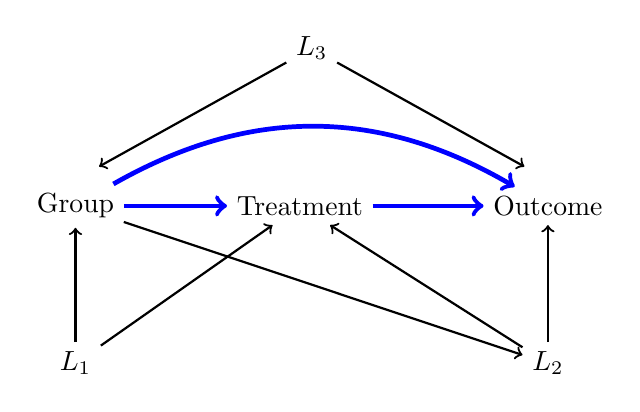
\begin{tikzpicture}[scale = 1] 
    \node at (0,0) {};
    \node at (1,1) {};
    
    \node[anchor = center, align = center] (g) at (0,-1) {Group};
    \node[anchor = center, align=center] (d) at (2.85,-1) {Treatment}; 
    \node[anchor = center, align=center] (y) at (6,-1) {Outcome};   
    \node[anchor = center, align=center] (l1) at (0, -3) {$L_1$};
    \node[anchor = center, align=center] (l2) at (6, -3) {$L_2$};
    \node[anchor = center, align=center] (l3) at (3, 1) {$L_3$};
    
    \draw[->, line width=0.6mm, blue] (g) to (d);
    \draw[->, line width=0.6mm, blue] (d) to (y);
    \draw[->, line width=0.6mm, blue] (g) to [bend left = 30] (y);  
    
    \draw[->, thick] (l1) to (g);  
    \draw[->, thick] (l1) to (d);  
    \draw[->, thick] (l2) to (d);  
    \draw[->, thick] (l2) to (y);  
    \draw[->, thick] (g) to (l2);  
    \draw[->, thick] (l3) to (0.3,-0.5);  
    \draw[->, thick] (l3) to (5.7,-0.5);  
\end{tikzpicture}
}
\subfigure[Group decomposition]
{
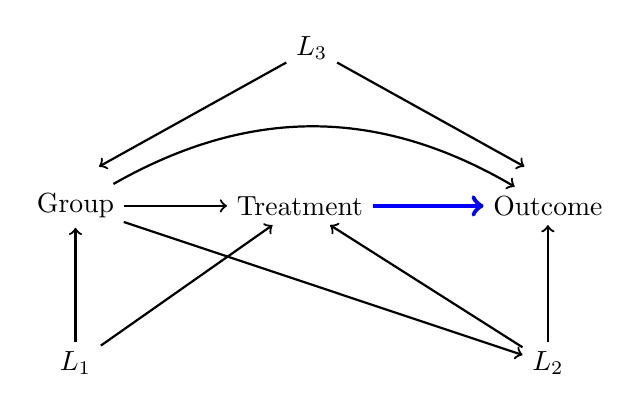
\begin{tikzpicture}[scale = 1]  
    \node at (0,0) {};
    \node at (1,1) {};
    
    \node[anchor = center, align = center] (g) at (0,-1) {Group};
    \node[anchor = center, align=center] (d) at (2.85,-1) {Treatment}; 
    \node[anchor = center, align=center] (y) at (6,-1) {Outcome};   
    \node[anchor = center, align=center] (l1) at (0, -3) {$L_1$};
    \node[anchor = center, align=center] (l2) at (6, -3) {$L_2$};
    \node[anchor = center, align=center] (l3) at (3, 1) {$L_3$};
    
    \draw[->, thick] (g) to (d);
    \draw[->, line width=0.6mm, blue] (d) to (y);
    \draw[->, thick] (g) to [bend left = 30] (y);  
    
    \draw[->, thick] (l1) to (g);  
    \draw[->, thick] (l1) to (d);  
    \draw[->, thick] (l2) to (d);  
    \draw[->, thick] (l2) to (y);  
    \draw[->, thick] (g) to (l2);  
    \draw[->, thick] (l3) to (0.3,-0.5);  
    \draw[->, thick] (l3) to (5.7,-0.5);  
\end{tikzpicture}
}

\caption{DAGs illustrating the difference in identification goals between causal mediation analysis and causal decomposition of group disparities. The highlighted edges are the paths each estimand seeks to identify. Causal mediation analysis aims to identify both the effects of group and treatment, hence requiring proper handling of all three types of confounders: $L_1$, $L_2$, and $L_3$. Our causal decomposition only needs to identify the effect of treatment, so only treatment-outcome confounders, i.e., $L_2$, are of concern.} \label{fig:DAG}

\end{figure}


\subsection{Relation to unconditional random equalization}
In recent years, a number of authors have proposed two variants of what we call the unconditional random equalization decomposition, which decomposes the observed disparity into two components. One is a reduction in disparity that can be eliminated by randomly reassign treatment $D$ so that the mean of $D$ becomes identical in both groups. The other is correspondingly a component of remaining disparity \citep{vanderweele_causal_2014, jackson_decomposition_2018, sudharsanan_educational_2021, lundberg_gap-closing_2022}. Like our approach, the random equalization decomposition seeks to identify the causal effect of $D$, not that of $G$. However, the random equalization decomposition is a two-way decomposition that contains less information than our four-way decomposition. Moreover, the reduction in disparity in random equalization combines the selection component and the prevalence component of the group disparity, impeding a clear interpretation.

%%%%% The random equalization decomposition was pioneered by \citet{vanderweele_causal_2014}. \citet{jackson_meaningful_2021} extended it to a conditional version, where the random equalization is only conceived within each level of some conditioning variables $\boldsymbol{Q}$. \citet{lundberg_gap-closing_2022} further proposed a slightly different estimand, where both group $a$ and group $b$ are given $D$ values randomly drawn from the entire sample. For the random equalization decomposition, estimators have been constructed based on regression \citep{vanderweele_causal_2014, jackson_decomposition_2018}, weighting \citep{jackson_meaningful_2021}, Monte Carlo integration \citep{sudharsanan_educational_2021}, as well as the doubly-robust augmented inverse probability weighting \citep{lundberg_gap-closing_2022}, which combines regression with weighting.  %%%%%

The first variant of the random equalization decomposition is defined in terms of a random equalization intervention that randomly assigns $D$ values of the advantaged group to the disadvantaged group.
Using the randomized intervention notation introduced above, Jackson and VanderWeele 
 (\citeyear{jackson_decomposition_2018}) decompose the observed group disparities into two components:
\begin{gather}
\E_a(Y)-\E_b(Y)=\underbrace{\E_a(Y)-\E_b \left(Y_{R(D \mid G=a)} \right)}_{\text{remaining disparity}} + \underbrace{\E_b \left(Y_{R(D \mid G=a)} \right)-\E_b(Y)}_{\text{reduction in disparity}}.  \nonumber 
\end{gather}
The reduction in disparity term indicates the extent to which the observed disparity would be reduced by the random equalization intervention. In the random equalization literature, this intervention is intended to quantify the contribution of the differential prevalence of $D$ across groups. 
However, the random equalization not only equalizes the treatment prevalence across groups, but also randomizes the treatment within group $b$, making any selection into treatment disappear in group $b$. As a consequence, the reduction in disparity equals the combination of the prevalence component and the group $b$ part of the selection component, i.e., $\E_b(\tau)[\E_a(D)-\E_b(D)]-\Cov_b(D, \tau)$, which follows from equation (\ref{eqt2}). This leads to an undesirable result: If group $a$ is an exact replicate of group $b$, the random equalization decomposition would still contain a non-zero reduction in disparity, as long as $\Cov_b(D, \tau) \neq 0$.

The second variant of the random equalization decomposition takes a somewhat different form \citep{lundberg_gap-closing_2022}, whose hypothetical intervention matches each individual in both groups with a random draw of $D$ from the pooled population. Hence, this variant of random equalization changes the $D$ values in both groups instead of only in the disadvantaged group as in the first variant. The reduction in disparity of this variant  mixes the prevalence component with the selection component, too. To show this, we first note that the outcome disparity can also be decomposed as such: 
\begin{align*}
&\phantom{{}={}} \E_a(Y)-\E_b(Y) \\
&= \E_a(Y_{0})-\E_b(Y_{0}) + \E(\tau)[\E_a(D)-\E_b(D)] \\
&\phantom{{}={}} + \E(D)[ \E_a(\tau) - \E_b(\tau)] + \Cov_a(D, \tau) - \Cov_b(D, \tau) \\
&\phantom{{}={}} - [P_a-P_b][\E_a(D) - \E_b(D)][\E_a(\tau)-\E_b(\tau)], 
\end{align*} 
where $\E(\tau)$ and $\E(D)$ are the overall ATE and treatment prevalence, $P_a$ and $P_b$ are the proportion of the population in group $a$ and group $b$.
And the remaining disparity in Lundberg's (\citeyear{lundberg_gap-closing_2022}) unconditional decomposition equals 
$\E_a(Y_{0})-\E_b(Y_{0}) + \E(D)[ \E_a(\tau) - \E_b(\tau)] \nonumber$. It then follows that the reduction in disparity in this case contains the selection component, $\Cov_a(D, \tau) -  \Cov_b(D, \tau)$, which does not involve the difference in treatment prevalence. The intuition is that in Lundberg's (\citeyear{lundberg_gap-closing_2022}) random equalization, both group $a$ and group $b$ would get random draws of $D$, thus  selection into treatment is eliminated in both groups, making $\Cov_a(D,\tau)=\Cov_b(D,\tau)=0$.

To conclude, the reduction in disparity in both variants of the random equalization decomposition is a mixture of the prevalent component and the selection component of group disparities. This is because its underlying intervention both equalizes and randomizes the treatment. In contrast, as discussed in Section 2.1,  the prevalence component in our decomposition is solely concerned with the disparity-reducing impact of an equalizing intervention and avoids the influence of a randomizing intervention. \footnote{This is also why the RIA of PIE can be translated to the prevalence component, but not to the reduction in disparity component in random equalization decompositions. Both the prevalence component and the RIA of PIE compare two quantities that likewise contain randomized $D$ values, so both estimands can represent the reduction in disparity resulting from a pure equalization intervention \emph{after} a randomization intervention.} If the goal is to capture the contribution of differential treatment prevalence to group disparities, one should prefer using the prevalence component in our decomposition.
 
\subsection{Conditional decomposition}
In this subsection, we derive a decomposition method where the corresponding intervention is conditional on a vector of variables $\boldsymbol{Q}$, which is temporally precedent to $D$. The conditional decomposition is useful as it  can shed light on the impact of normatively more desirable or realistically more feasible interventions, when the unconditional intervention appears less so \citep{jackson_meaningful_2021}.  
Assuming that the the support of $\Q$ is the same in the two groups and still under the SUTVA assumption (A.1),
\begin{align}
    \E_a(Y)-\E_b(Y) &= \underbrace{\E_a(Y_0)-\E_b(Y_0)}_{\text{baseline}} \nonumber \\
    &\phantom{{}={}} + \underbrace{\int [\E_a(D \mid \Q=\q)-\E_b(D \mid \Q=\q)]\E_b(\tau \mid \Q=\q) f_b(\q) \dd \q}_{\text{conditional prevalence}} \nonumber \\
    &\phantom{{}={}} + \underbrace{\int [\E_a(\tau \mid \Q=\q)-\E_b(\tau \mid \Q=\q)] \E_a(D \mid \Q=\q) f_a(\q) \dd \q}_{\text{conditional effect}} \nonumber \\
    &\phantom{{}={}} + \underbrace{\E_a[\Cov_a(D, \tau \mid \Q)] - \E_b[\Cov_b(D, \tau \mid \Q)}_{\text{conditional selection}}] \nonumber \\
    &\phantom{{}={}} + \underbrace{\int \E_a(D \mid \Q=\q) \E_b(\tau \mid \Q=\q) [f_a(\q)-f_b(\q)] \dd \q}_{\text{$\Q$ distribution}}.
\end{align}

From an interventional perspective, now the conditional prevalence, effect, and selection components indicate the disparity-reducing impacts of equalizing the corresponding group characteristics within levels of $\Q$. These conditional equalizations are often substantively weaker than the marginal equalizations encoded in equation (\ref{eqt1}). For example, if marginally equalizing college access across SES backgrounds appears to be either normatively or practically too strong, a weaker intervention that equalizes college access within levels of prior achievement may still be of interest. In general, the conditional decomposition allows researchers to incorporate prior information about subjects when designing a re-distribution of treatments or their effects. Additionally, the ``$\Q$ distribution'' component captures the between-$\Q$ disparity, as opposed to within-$\Q$ disparities reflected in other components, but it should not be interpreted causally, as we do not make any causal identification assumptions for $\Q$.

Similar to the unconditional case, we can also interpret the conditional decomposition from an interventional perspective using the randomized intervention notation. 
Let $\E_g(Y_{R(D \mid G=g',\Q)})$ be the mean potential outcome of group $g$ when members of group $g$ were given treatment values randomly drawn from members of group $g'$ who share the same $\Q$ values with them. We can rewrite this mean potential outcome as such:
\begin{align}
    \E_g(Y_{R(D \mid G=g',\Q)}) = \E_g(Y_0) + \int \E_g(\tau \mid \Q=\q) \E_{g'}(D \mid \Q=\q) f_g(\q) \dd \q.
\end{align}
It then follows that components of the conditional decomposition can be written in the randomized intervention notation:
\begin{align}
    \E_a(Y)-\E_b(Y)-[\E_a(Y_{R(D \mid G=a,\Q)})-\E_b(Y_{R(D \mid G=b,\Q)})] &= \text{conditional selection} \nonumber \\
    \E_b(Y_{R(D \mid G=a,\Q)}) - \E_b(Y_{R(D \mid G=b,\Q)}) &= \text{conditional prevalence} \nonumber \nonumber \\
    \E_a(Y_{R(D \mid G=a,\Q)}) - \E_b(Y_{R(D \mid G=a,\Q)}) &= \text{conditional effect} + \text{conditional selection} \nonumber \\
    &\phantom{{}={}} + \text{$\Q$ distribution}.
\end{align}

Therefore, a sequential intervention again underlies our conditional decomposition. In the first step, the distribution of treatment is randomized within each $\Q$ level for members of both groups. The reduction in disparity resulting from this step is then the conditional selection component. The second step is an equalization intervention on the top of the previous randomization step. For the second step, the pre-intervention disparity is $\E_a(Y_{R(D \mid G=a,\Q)})-\E_b(Y_{R(D \mid G=b,\Q)})$, and the post-intervention disparity is $\E_a(Y_{R(D \mid G=a,\Q)}) - \E_b(Y_{R(D \mid G=a,\Q)})$. Then it becomes clear that the conditional prevalence component is the reduction in disparity brought about by giving group $b$ random draws of treatment from group $a$ within $\Q$ levels. What would remain after the sequential intervention is the sum of the conditional effect, the conditional selection, and the $\Q$ distribution components.

Similar to the (unconditional) random equalization decomposition, \citet{jackson_meaningful_2021} and \citet{lundberg_gap-closing_2022} proposed two variants of what can be called the conditional random equalization decomposition (CRED), which decomposes outcome disparities into a reduction in disparity component and a remaining disparity component. The hypothetical intervention underlying the CRED is a random re-distribution of treatment values within $\Q$ levels such that treatment prevalence would be equalized within $\Q$ levels. Analogous to the unconditional case, we show that the reduction in disparity component in both variants of CRED conditionally mixes the prevalence component with the selection component, thus the conditional prevalence component in our decomposition should be preferred for its clearer interpretation. 

In Jackson's (\citeyear{jackson_meaningful_2021}) version of the CRED, the reduction in disparity is $\E_b(Y_{R(D \mid G=a, \Q)})-\E_b(Y)$, which we can rewrite as 
\begin{gather}
\int  [\E_a(D \mid \Q=\q) - \E_b(D \mid \Q=\q)] \E_b(\tau \mid \Q=\q) f_b(\q) \dd \q - \E_b[\Cov_b(D, \tau \mid \Q)]. 
\end{gather}
Therefore, the reduction in disparity is a mixture of the conditional prevalence component and part of the conditional selection component. Namely, it captures not only differential $D$ prevalence within $\Q$ levels, but also the extent of conditional selection into treatment in group $b$. Intuitively, this is because the CRED involves both a conditional equalization and a conditional randomization, and the randomization part eliminates effect-based selection into treatment conditional on $\Q$ in group $b$. 

A similar case can be shown for the reduction in disparity in the CRED of \citet{lundberg_gap-closing_2022}.
\begin{align}
&\phantom{{}={}} \E_a(Y)-\E_b(Y) \nonumber \\ 
&\phantom{{}={}} \left\lbrace \E_a[\Pro(D=0 \mid \Q) Y_0 + \Pro(D=1 \mid \Q) Y_1] - \E_b[\Pro(D=0 \mid \Q) Y_0 + \Pro(D=1 \mid \Q) Y_1] \right\rbrace \nonumber \\
&= \E_a[\Cov_a(D,\tau \mid \Q)] - \E_b[\Cov_b(D,\tau \mid \Q)] + \int [\E_a(D \mid \Q=\q) - \E_b(D \mid \Q=\q)] \nonumber \\
&\phantom{{}={}} [\E_a(\tau \mid \Q=\q)f_a(\q)\Pro(G=b \mid \Q=\q) + \E_b(\tau \mid \Q=\q)f_b(\q)\Pro(G=a \mid \Q=\q)] \dd \q,
\end{align}
where the left hand side is the reduction in disparity in Lundberg's CRED. Hence, the reduction in disparity again involves both a term for differential prevalence within $\Q$ levels and our conditional selection component. The CRED in this case posits an intervention where equalization across groups and randomization in both groups are conducted at each $\Q$ level. Consequently, both differential prevalence and differential selection would be reduced to zero conditional on $\Q$. Distinct from both versions of the CRED, the component of conditional prevalence in our decomposition is solely a measure of the impact of a conditional equalization intervention. By implication, only our conditional prevalence component can be interpreted as a pure measure of the contribution of differential treatment prevalence within $\Q$ levels to  outcome disparities. 


\section{Estimation and Inference}
In this paper, we focus on identifying the components of our decompositions using two standard assumptions as follows. \footnote{Our unconditional decomposition can also be identified using the Marginal Treatment Effect approach based on an instrumental variable \citep{heckman_structural_2005, zhou_heterogeneous_2020}, as identifying group-specific ATTs and ATEs is sufficient.}
\begin{itemize}
    \item[] (A.2) (Conditional ignorability) $Y_d \indep D \mid \X=\x, \Q=\q, G=g$, $\forall d, \x, \q, g$;
    \item[] (A.3) (Overlap) $0 < \E(D \mid \X=\x, \Q=\q, G=g) <1$, $\forall \x, \q, g$,
\end{itemize}
where $\Q$ is omitted for the unconditional decomposition. 
We develop nonparametric and efficient estimators for components of our unconditional and conditional decompositions 
\footnote{Various regression, weighting, or matching estimators can also be used. In particular, under constant treatment effect, the prevalence component in the unconditional decomposition can be estimated using the traditional ``product method'' for the indirect effect of $G$ through $D$ on $Y$ \citep{baron_moderator-mediator_1986}. This again explicates the kinship between our decomposition and the traditional mediation analysis. }. 
These estimators are ``one-step'' estimators based on the EIFs of the decomposition components, which removes the bias from naive substitution estimators \citep{bickel_efficient_1998, van_der_vaart_asymptotic_2000,hines_demystifying_2022}. The estimators contain some nuisance functions, which can be estimated using flexible ML methods coupled with cross-fitting. Under specified conditions, our estimators are $\sqrt{n}$-consistent, asymptotically normal, and semiparametrically efficient. Thus, we are able to construct asymptotically accurate Wald-type confidence intervals and hypothesis tests. Our estimators also have certain double robustness properties.  


To introduce the EIFs, we define the following functions:
\begin{align*}
    \mu(d,\X,\Q, g)&=\E(Y \mid D, \X, \Q, G=g) \\
    \pi(d,\X, \Q, g) &= \Pro(D=d \mid \X, \Q, G=g) \\
    p_g &= \Pro(G=g) \\
    p_g(\Q) &= \Pro(G=g \mid \Q).
\end{align*}
Below, we use $\xi$ to denote the estimands (decomposition components), $\phi$ to denote the EIFs, and $\Psi$ to denote the resulting one-step estimators. 

\subsection{The unconditional decomposition}
All components of the unconditional decomposition are simple linear combinations of the total disparity and two generic functions evaluated at appropriate values of $d$, $g$, and $g'$: $\xi_{dg} \defeq \E \left(Y_d \mid G=g  \right)$ and $\xi_{dgg'} \defeq \E \left(Y_d \mid G=g \right)\E \left(D \mid G=g' \right)$. The relationship between components of the unconditional decomposition and the generic functions are as follows:
\begin{align*}
    \text{Baseline} &= \xi_{0a}-\xi_{0b}  \\
    \text{Prevalence} &= \xi_{1ba}-\xi_{0ba}-\xi_{1bb}+\xi_{0bb} \\
    \text{Effect} &= \xi_{1aa}-\xi_{0aa} - \xi_{1ba}+\xi_{0ba} \\
    \text{Selection} &= \text{Total} - \text{Baseline} - \text{Prevalence} - \text{Effect} .
\end{align*}
Hence, the EIFs and one-step estimators for the decomposition components directly follow from the EIFs and one-step estimators of $\xi_{dg}$ and $\xi_{dgg'}$. The estimation of the total disparity is straightforward, so we will only present the estimators for $\xi_{dg}$ and $\xi_{dgg'}$. In addition, these generic functions also provide a basis for estimating Jackson's (\citeyear{jackson_decomposition_2018}) version of the unconditional equalization estimand, since its reduction in disparity component can be represented as $\xi_{0b} + \xi_{1ba}-\xi_{0ba}-\E_b(Y)$. Under assumptions A.1, A.2, and A.3, $\xi_{dg}$ and $\xi_{dgg'}$ can be identified as the following functions:
\begin{align*}
    \xi_{dg} &= \E \left[\mu(d,\X,g) \mid G=g \right] \\
    \xi_{dgg'} &= \E \left[\mu(d,\X,g) \mid G=g \right] \E \left[D \mid G=g' \right].
\end{align*}

Given the identification results above, we derive the EIFs for $\xi_{dg}$ and $\xi_{dgg'}$, which provide the basis for flexible yet efficient one-step estimators.
\begin{prop}
Under assumptions A.1, A.2, and A.3, the EIF of $\xi_{dg}$ is
$$\phi_{dg}(Y,\X) \defeq \frac{\one(G=g)}{p_g} \left\{ \frac{\one(D=d)}{\pi(d, \X,g)} [Y-\mu(d,\X,g)] + \mu(d,\X,g) - \xi_{dg} \right\},$$ 
and the EIF of $\xi_{dgg'}$ is
\begin{align*}
    \phi_{dgg'}(Y,\X) &\defeq \frac{\one(G=g)}{p_g}  \left\{\frac{\one(D=d)}{\pi(d,\X,g)}[Y-\mu(d,\X,g)] + \mu(d,\X,g) \right\} \E \left(D \mid G=g' \right) \\
    &\phantom{{}={}} + \frac{\one(G=g')}{p_{g'}} \E \left(Y_d \mid G=g \right) \left[D - \E \left(D \mid G=g' \right) \right] - \frac{\one(G=g)}{p_g} \xi_{dgg'}.
\end{align*}
In appendix B, we also derive the EIFs for the general case with survey weights for both unconditional and conditional decompositions. 
\end{prop}
It follows that the one-step estimators are
\begin{align*}
    \Psi_{dg}(Y,\X) &\defeq \frac{1}{n} \sum \frac{\one(G=g)}{p_g} \left\{ \frac{\one(D=d)}{\pi(d, \X,g)} [Y-\mu(d,\X,g)] + \mu(d,\X,g)\right\} \\
    \Psi_{dgg'}(Y,\X) &\defeq \frac{1}{n} \sum \frac{\one(G=g)}{p_g}  \left\{\frac{\one(D=d)}{\pi(d,\X,g)}[Y-\mu(d,\X,g)] + \mu(d,\X,g) \right\} \E \left(D \mid G=g' \right).
\end{align*}
For any $g$ and $d$, there are two nuisance functions, $\pi(d,\X,g)$, and $\mu(d,\X,g)$. In order to relax the conditions required of nuisance function estimators \citep{kennedy_semiparametric_2022, chernozhukov_double/debiased_2018}, we use cross-fitting to estimate all nuisance functions. In particular, we first divide the sample randomly into two subsamples. Then we fit the nuisance functions using each subsample. Finally, we evaluate the fitted nuisance functions using data not in the subsample that is used to fit the functions. In practice, to improve the finite-sample performance of the estimator, we may stabilize the weights by dividing $\frac{\one(D=d)}{\pi(d,\X,g)}$ by its sample average.  

To study the asymptotic behavior of the one-step estimators for the unconditional decomposition, we invoke three additional sets of assumptions, \footnote{Throughout this paper, the consistent estimation of $p_g$ and $\E(D \mid G=g), \forall g,$ are left implicit.} which are consistent with assumptions required for the double ML estimator of ATE \citep{kennedy_semiparametric_2022, chernozhukov_double/debiased_2018}. We let $\| \cdot \|$ denote the $L_2$-norm. 

(A.4.a) (Boundedness): With probability 1, $\hat{\pi}(d,\X,g) \geq \eta$, $\pi(d,\X,g) \geq \eta$, and $|Y-\hat{\mu}(d,\X,g)| \leq \zeta$, for some $\eta>0$ and some $\zeta < \infty$, $\forall d, g$.

(A.5.a) (Consistency):  $\| \hat{\mu}(d,\X,g) - \mu(d,\X,g) \| =o_p(1)$ and $\| \hat{\pi}(d,\X,g) - \pi(d,\X,g) \| =o_p(1)$, $\forall d, g$.

(A.6.a) (Convergence rate):  $\|\hat{\pi}(d,\X,g)-\pi(d,\X,g)\| \|\hat{\mu}(d,\X,g)-\mu(d,\X,g)\|=o_p(n^{-1/2})$, $\forall d, g$.

\begin{prop}
Under assumptions A.1, A.2, A.3, A.4.a, A.5.a, and A.6.a, the one step estimators for components of the unconditional decomposition are asymptotically normal and semiparametrically efficient, i.e., $\sqrt{n}(\Psi_{dg} - \xi_{dg}) \xrightarrow{d} \mathcal{N}(0, \sigma^2_{dg})$, and $\sqrt{n}(\Psi_{dgg'} - \xi_{dgg'}) \xrightarrow{d} \mathcal{N}(0, \sigma^2_{dgg'})$, where $\sigma^2_{dg}=\E[\phi_{dg}(Y,\X)^2]$ and $\sigma^2_{dgg'}=\E[\phi_{dgg'}(Y,\X)^2]$ are the respective semiparametric efficiency bounds. 
\end{prop}
Assumptions A.4.a through A.6.a are mild in the sense that it is often possible to use ML to estimate the nuisance functions and still attain desirable asymptotic properties. These asymptotic properties also carry over from $\Psi_{dg}$ and $\Psi_{dgg'}$ to the estimators of the decomposition components. We estimate $\sigma^2_{dg}$ and $\sigma^2_{dgg'}$ using the  averages of squared estimated EIFs. The asymptotic distributions can then be used to construct hypothesis testing and confidence intervals. For example, a Wald-style $1-\alpha$ confidence interval for the prevalence component is $$\Psi_{1ba}-\Psi_{1bb}-\Psi_{0ba}+\Psi_{0bb} \pm z_{1-\alpha/2} \cdot \frac{1}{n} \left[\sum  \left(\hat{\phi}_{1ba}-\hat{\phi}_{1bb}-  \hat{\phi}_{0ba}+\hat{\phi}_{0bb}\right)^2 \right]^{1/2}.$$ Furthermore, our estimators also have a doubly robustness property. 

\begin{prop}[Double robustness]
Either consistent estimation of $\mu(d,\X,g)$ or $\pi(d,\X,g)$ for all $d$ and $g$ is sufficient for the consistency of $\Psi_{dg}$ and $\Psi_{dgg'}$.  
\end{prop}
Hence, our unconditional decomposition estimator essentially only requires the same conditions as the classic augmented inverse probability weighting estimator for ATE \citep{robins_estimation_1994, hirano_efficient_2003} to be consistent. 

\subsection{The conditional decomposition}
Relative to the unconditional case, we only need to additionally consider one generic function:
$$\xi_{dgg'g''} \defeq \E \left[\E \left(Y_d   \mid \Q, g \right) \E \left(D \mid \Q, g' \right) \mid G=g'' \right],$$
where $(d, g, g', g'')$ is any combination of treatment status and group memberships out of  8 possible combinations. The relationship between components of the conditional decomposition and the generic functions are as follows:
\begin{align*}
    \text{Baseline} &= \xi_{0a}-\xi_{0b}  \\
    \text{Conditional Prevalence} &= \xi_{1bab}-\xi_{0bab}-\xi_{1bbb}+\xi_{0bbb} \\
    \text{Conditional Effect} &= \xi_{1aaa}-\xi_{0aaa} - \xi_{1baa}+\xi_{0baa} \\
    \Q \text{ Distribution} &= \xi_{1baa}-\xi_{0baa} - \xi_{1bab}+\xi_{0bab} \\
    \text{Conditional Selection} &= \text{Total} - \text{Baseline} \\
    &\phantom{{}={}} - \text{Conditional Prevalence} - \text{Conditional Effect} - \Q \text{ Distribution}.
\end{align*}
Hence, in this subsection, we focus on the inference of $\xi_{dgg'g''}$. The EIFs,  one-step estimators, and their asymptotic distributions for components of the conditional decomposition will then straightforwardly follow. Moreover, we thereby also provide nonparametric inference for the reduction in disparity component in the CRED of \citet{jackson_meaningful_2021}, which can be represented as $\xi_{0b}+\xi_{1bab}-\xi_{0bab}-\E_b(Y)$.
Under assumptions A.1, A.2, and A.3, we identify $\xi_{dgg'g''}$ as $$\E \left\{\E \left[ \E(Y \mid d,\X,\Q,g)   \mid \Q, g \right] \E \left(D \mid \Q, g' \right) \mid G=g'' \right\}.$$

\begin{prop}
Under assumptions A.1, A.2, and A.3, the EIF of $\xi_{dgg'g''}$ is 
\begin{align*}
     &\phantom{{}={}} \phi_{dgg'g''}(Y,\X,\Q) \\
    &=\frac{\one(G=g'')}{p_{g''}} \left[ \E \left(Y_d \mid \Q, g \right) \E \left(D \mid \Q, g' \right) - \xi_{dgg'g''} \right] \\
    &\phantom{{}={}} + \frac{\one(G=g) p_{g''}(\Q)}{p_g(\Q)p_{g''}} \left\{ \frac{\one(D=d)}{\pi(d,\X,\Q,g)} [Y-\mu(d,\X,\Q,g)]+\mu(d,\X,\Q,g) - \E \left(Y_d \mid \Q,g \right) \right\} \E \left(D \mid \Q,g' \right) \\
    &\phantom{{}={}} + \frac{\one(G=g')p_{g''}(\Q)}{p_{g'}(\Q)p_{g''}} \left[ D-\E \left(D \mid \Q, g' \right) \right] \E\left( Y_d \mid \Q, g \right).
\end{align*}
The general case with survey weights is derived in Appendix B.
\end{prop}
We again construct one-step estimators based on the EIFs. 
\begin{align*}
    &\phantom{{}={}} \Psi_{dgg'g''}(Y,\X,\Q) \\
    &=\frac{\one(G=g'')}{p_{g''}} \E \left(Y_d \mid \Q, g \right) \E \left(D \mid \Q, g' \right) + \frac{\one(G=g')p_{g''}(\Q)}{p_{g'}(\Q)p_{g''}} \left[ D-\E \left(D \mid \Q, g' \right) \right] \E\left( Y_d \mid \Q, g \right) \\
    &\phantom{{}={}} + \frac{\one(G=g) p_{g''}(\Q)}{p_g(\Q)p_{g''}} \left\{ \frac{\one(D=d)}{\pi(d,\X,\Q,g)} [Y-\mu(d,\X,\Q,g)]+\mu(d,\X,\Q,g) - \E \left(Y_d \mid \Q,g \right) \right\} \E \left(D \mid \Q,g' \right).
\end{align*}
For this estimator, there are five nuisance functions: $p_g(\Q)$, $\pi(d,\X,\Q,g)$, $\mu(d,\X,\Q,g)$, $\E(D \mid \Q, G=g)$, and $\E(Y_d \mid \Q,g)$, for any $d$ and $g$. We cross-fit these nuisance functions using nonparametric methods. This estimator can be weight-stabilized by dividing $\frac{\one(D=d)}{\pi(d,\X,\Q,g)}$, $\frac{\one(G=g')p_{g''}(\Q)}{p_{g'}(\Q)p_{g''}}$, and $\frac{\one(G=g)p_{g''}(\Q)}{p_g(\Q)p_{g''}}$ by their respective sample averages. The estimation of $\E(Y_d \mid \Q,g)=\E[\mu(d,\X,\Q,g) \mid \Q,g]$ requires a more involved procedure. We adopt a pseudo-outcome approach \citep[e.g.,][]{van_der_laan_statistical_2006,semenova_debiased_2021}, where the pseudo outcome is defined as the decentered EIF for $\E(Y_d)$, i.e., 
$$ \frac{\one(D=d)}{\pi(d, \X,G)} [Y-\mu(d,\X,G)] + \mu(d,\X,G).$$
We first estimate $\pi(d, \X,G)$ and $\mu(d,\X,G)$ in the pseudo outcome for each individual within two random subsamples of the data \emph{without} cross-fitting. Then, using nonparametric regression methods, we flexibly predict the estimated pseudo outcome using $\Q$ and $G$. The resulting predictions become estimates of $\E(Y_d \mid \Q,g)$. We use cross-fitting in the second step, i.e., when one subsample is used to fit $\E(Y_d \mid \Q,g)$, the $\Q$ and $G$ values of the other subsample are plugged in to obtain predictions. Using this procedure, we ensure that the fitting of the function $\E(Y_d \mid \Q,g)$, which relies on estimating the pseudo outcome, is done separately in each subsample. 

The asymptotic theory of the one-step estimator for $\xi_{dgg'g''}$ is less general than the theories for $\xi_{dg}$ and $\xi_{dgg'}$, in that some conditions differ by the specific configuration of $g, g'$ and $g''$. Note that  $g=g''$ for the conditional prevalence component, and $g'=g''$ for the conditional effect component. For $\sqrt{n}$-consistency, asymptotic normality, and efficiency, we need three assumptions. 

(A.4.b) (Boundedness): With probability 1,  $\hat{\pi}(d,\X,\Q,g) \geq \eta$, $\pi(d,\X,\Q,g) \geq \eta$, $\hat{p}_g(\Q) \geq \eta$, $p_g(\Q) \geq \eta$, 
$|Y-\hat{\mu}(d,\X,\Q,g)| \leq \zeta$, 
$|Y-\mu(d,\X,\Q,g)| \leq \zeta$, 
$|\mu(d,\X,\Q,g)| \leq \zeta$,
$|\E(Y_d \mid \Q,g)| \leq \zeta$, and $\left| \frac{\hat{p}_g(\Q)}{\hat{p}_{g'}(\Q)} \right| \leq \zeta$, for some $\eta>0$ and $\zeta < \infty$, $\forall d,g,g'$.

(A.5.b) (Consistency): $\| \hat{\mu}(d,\X,\Q,g) - \mu(d,\X,\Q,g) \| =o_p(1)$, $\| \hat{\pi}(d,\X,\Q,g) - \pi(d,\X,\Q,g) \| =o_p(1)$, $\left\| \hat{\E}(Y_d \mid \Q,g) - \E(Y_d \mid \Q,g) \right\| =o_p(1)$, $\left\| \hat{\E}(D \mid \Q,g) - \E(D \mid \Q,g) \right\| =o_p(1)$, and $\left\| \hat{p}_g(\Q) -p_g(\Q) \right\|=o_p(1)$, $\forall d,g$.

(A.6.b) (Convergence rate): $\left\|\hat{\pi}(d,\X,\Q,g)-\pi(d,\X,\Q,g) \right\| \|\hat{\mu}(d,\X,\Q,g)-\mu(d,\X,\Q,g)\|=o_p(n^{-1/2})$, $\left\| \one(G=g) \E(Y_d \mid \Q,g) - \one(G=g')\frac{\hat{p}_{g}(\Q)}{\hat{p}_{g'}(\Q)} \hat{\E}( Y_d \mid \Q, g ) \right\| \left\| \hat{\E}(D \mid \Q, g') - \E(D \mid \Q, g') \right\| = o_p(n^{-1/2})$, and $\left\| \one(G=g') \E(D \mid \Q,g') - \one(G=g) \frac{\hat{p}_{g'}(\Q) }{\hat{p}_g(\Q) } \hat{\E}(D \mid \Q,g') \right\| \left\| \hat{\E}(Y_d \mid \Q,g) - \E(Y_d \mid \Q,g)  \right\| = o_p(n^{-1/2})$, $\forall d,g,g'$.

\begin{prop}
Under assumptions A.1, A.2, A.3, A.4.b, A.5.b, and A.6.b, the one step estimator for components of the conditional decomposition is asymptotically normal and semiparametrically efficient, i.e., $\sqrt{n} \left( \Psi_{dgg'g''} - \xi_{dgg'g''} \right) \xrightarrow{} \mathcal{N}(0, \sigma^2_{dgg'g''})$, where $\sigma^2_{dgg'g''}=\E[\phi_{dgg'g''}(Y,\X,\Q)^2]$ is the semiparametric efficiency bound.
\end{prop}
Some further insights can be gained about the second and third convergence rate assumptions . For a specific $\xi_{dgg'g''}$, first, when $g=g'=g''$, $\left\| \hat{\E}\left( Y_d \mid \Q, g \right) - \E(Y_d \mid \Q,g)  \right\| \left\| \hat{\E}(D \mid \Q, g) - \E(D \mid \Q, g)  \right\| = o_p(n^{-1/2})$ is sufficient. Hence, we obtain a form of rate double robustness with respect to $\E(Y_d \mid \Q,g)$ and $\E(D \mid \Q, g)$. Second, when $g= g'' \neq g'$, the following set of conditions is sufficient: for a constant $\zeta>0$, $\frac{\hat{p}_g(\Q)}{\hat{p}_{g'}(\Q)} \leq \zeta$ with probability 1, $\left\| \hat{\E}(D \mid \Q, g') - \E(D \mid \Q, g') \right\|=o_p(n^{-1/2})$, and $ \left\| \hat{\E}\left( Y_d \mid \Q, g \right) - \E(Y_d \mid \Q,g) \right\|=o_p(1)$. Third, when $g'=g'' \neq g$, a sufficient set is: for a constant $\zeta>0$, $ \frac{\hat{p}_{g'}(\Q)}{\hat{p}_{g}(\Q)} \leq \zeta$ with probability 1, $\left\| \hat{\E}(D \mid \Q, g') - \E(D \mid \Q, g') \right\|=o_p(1)$, and $\left\| \hat{\E}\left( Y_d \mid \Q, g \right) - \E(Y_d \mid \Q,g)  \right\|=o_p(n^{-1/2})$. Therefore, the assumption is weaker for the inference of the conditional prevalence component, which is also the case for Theorem 6 below.

\begin{prop}[Double robustness]
Assuming consistent estimation of $\E(D \mid \Q, g), \forall g$, for a $\xi_{dgg'g''}$, if $g=g''$, either consistent estimation of $\mu(d,\X,g)$ or $\pi(d,\X,g)$ is sufficient for the consistency of $\Psi_{dgg'g''}$; If $g \neq g''$, if, additionally, the consistent estimation of $\E(Y_d \mid \Q,g)$ is doubly robust with respect to $\mu(d,\X,g)$ and $\pi(d,\X,g)$, then $\Psi_{dgg'g''}$ is still doubly robust with respect to $\mu(d,\X,g)$ and $\pi(d,\X,g)$.
\end{prop}
Note that consistent estimation of $\hat{p}_g(\Q)$ is not required for the consistency of $\Psi_{dgg'g''}$. The double robustness condition for $\E(Y_d \mid \Q,g)$ in the case of $g \neq g''$ motivates our pseudo-outcome estimator of $\E(Y_d \mid \Q,g)$, which is built on both $\mu(d,\X,\Q,g)$ and $\pi(d,\X,\Q,g)$.

We have released an R package named cgdg to implement both the unconditional and conditional decompositions. It offers various options for nuisance function estimation, including various ML methods, a parametric option with linear and logistic regressions, and an option that allows users to manually plug in nuisance function estimates. The cdgd package can be installed from Github using \url{devtools::install_github("ang-yu/cdgd")}.


\section{Case study}
\subsection{Overview}
We apply our causal decomposition to investigate the role of college graduation in intergenerational income mobility in the United States. We estimate both the unconditional and conditional decomposition. We focus on the unconditional decomposition in the main text, since it allows us to more closely engage the previous social science literature. We discuss results for the conditional decomposition in Appendix F, which also has important policy implications. In this empirical setting, groups, $G$, are defined by parental income, the outcome, $Y$, is adult income, and treatment, $D$, is college graduation. 
Previous research has touched upon the components of our unconditional decomposition to various degrees, but this is the first study to comprehensively evaluate the three distinct ways in which college graduation might contribute to the intergenerational transmission of income advantages. 

The baseline component represents the part of the income attainment disparity that is unaccounted for by the multifaceted role of a college credential. Apart from college completion, parental income is associated with a variety of pre-college characteristics that have bearings on income attainment, such as academic achievement, cognitive skills, and noncognitive traits in adolescence \citep{reardon_widening_2011, heckman_effects_2006, farkas_cognitive_2003}. Any intervention imposed on the credentialing process in college cannot eliminate the influence of these characteristics on adult income.

%For example, people from more privileged  background may benefit from social and cultural capital passed on within their families hence would obtain higher incomes in adulthood regardless of formal educational attainment. Higher socioeconomic origin may also be conducive to advantages in assortative mating, which can improve income prospects. Income inequalities in cognitive and noncognitive abilities prior to post-secondary education may also be a channel of intergenerational income association that operates independently of the acquisition of college credential.

Resembling the prevalence component in our decomposition, education has been construed by social scientists as a mediator of the intergenerational reproduction of SES inequalities (\citealp[chapter 4 \& 5]{blau_american_1978}; \citealp[p.255-9]{featherman_opportunity_1978}; \citealp{ishida_class_1995}; \citealp{breen_educational_2010}). In particular, a large and increasing income gap in college graduation has been documented \citep{ziol-guest_parent_2016, bailey_gains_2011}. Using models that do not have causal and prescriptive implications, social scientists have attributed income persistence specifically to inequality in college completion \citep{bloome_educational_2018}. 

There is also an active literature on effect heterogeneity of college on SES attainment by SES origin, which underpins our effect component. Brand et al. (\citeyear{brand_uncovering_2021}) and Cheng et al. (\citeyear{cheng_heterogeneous_2021}) found that the college premiums on wage and income outcomes are larger for people who are economically disadvantaged during adolescence. However, Zhou (\citeyear{zhou_equalization_2019}) and Fiel (\citeyear{fiel_great_2020}) found only insignificant heterogeneity in the effect of college completion on income by parental income. However, these works did not evaluate the extent to which income disparities can be attributed to groupwise differential effects of college.

Finally, the literature on college effects on later SES status has yielded mixed findings regarding whether selection on the treatment effect is positive or negative overall in the US. Brand and Xie (\citeyear{brand_who_2010}) and Brand et al. (\citeyear{brand_uncovering_2021}) concluded that there is positive selection into college. However, Breen et al. (\citeyear{breen_heterogeneous_2015}) warned that Brand and Xie's (\citeyear{brand_who_2010}) result may be biased from unobserved confounding. The instrumental variable analysis of Heckman et al. (\citeyear{heckman_returns_2018}), on the other hand, reveals positive selection. This line of inquiry does not estimate group-specific selection patterns, hence missing the linkage between group-differentiated selection component and outcome disparities. In Appendix E, we clarify and synthesize the differences and connections between various concepts of `selection into college' in the social science literatures. 

\subsection{Data, variables and estimation details}
We analyze the National Longitudinal Survey of Youth 1979 (NLSY79), which is nationally representative for a cohort of young men and women who were born between 1957 and 1964 and were living in the United States at the baseline survey in 1979.
We  limit the analysis to respondents who were between 14 to 17 years old in 1979 to assure that income origin is measured prior to the time at which respondents might have had a chance to graduate from college. 

We contrast income-origin groups defined as the top and bottom quartiles of family incomes averaged over the first three waves of the survey (1979, 1980, and 1981), divided by the square root of the family size. The respondents were 14 to 20 years old during that time. The treatment variable is a binary indicator of whether the respondent graduates from college by the age of 31. We measure the outcome by the percentile rank of adult income, averaged over five survey waves between age 35 and 44, again divided by the square root of family size. For the conditional decomposition, we define $\Q$ as the Armed Forces Qualification Test (AFQT) score measured in 1980, which reflects academic achievement in high school. 

Covariates include gender, race, parental education, parental presence, number of siblings, urban residence, own educational expectation, friends' educational expectations, influential person's attitude regarding the respondent's college education, AFQT score, age at baseline survey, the Rotter locus of control scale score, the Rosenberg esteem item response score, language spoken at home, SMSA residence, living with mother, school curriculum, school satisfaction, foreign-born parents, region of residence, and mother's working status. 

We fit the nuisance functions using three alternative ML methods, Gradient Boosting Machine (GBM), Neural Networks and Random Forests, for which we use 10-fold cross-validation to tune hyper-parameters. For comparison, we also fit the nuisance functions using parametric regressions. For outcome models, we use linear regressions with all two-way interactions between the group indicator and baseline covariates, along with the constituting main effects. For propensity score models and models predicting $G$, the covariates are entered linearly. \footnote{Code for this analysis is posted at \url{https://github.com/ang-yu/causal_decomposition_case_study}.}

\subsection{Results}
% Sun Feb 12 22:16:09 2023
\begin{table}[ht]
\centering
\caption{Unconditional Decomposition Estimates} 
\begin{tabular}{lllll}
  \hline
   & GBM & Neural Networks & Random Forests & Parametric \\ 
  \hline
  Total & $0.286^{***}$ & $0.286^{***}$ & $0.286^{***}$ & $0.286^{***}$  \\ 
  Baseline & $0.276^{***}$ & $0.248^{***}$ & $0.255^{***}$ & $0.250^{***}$ \\ 
  Prevalence & $0.116^{***}$ & $0.123^{***}$ & $0.099^{***}$ & $0.070^{***}$ \\ 
  Effect & $0.053^{*}$ & $-0.008$ & $0.068^{*}$ & $-0.033$ \\ 
  Selection & $-0.160^{***}$ & $-0.077^{***}$ & $-0.137^{***}$ & $-0.001$ \\ 
  Jackson's reduction in disparity & $0.018$ & $0.066^{***}$ & $0.045^{***}$ & $0.069^{***}$ \\ 
   \hline
  \multicolumn{5}{l} {\makecell{Note: P value $<$ 0.05: *, $<$ 0.01: **, $<$ 0.001: ***. Weight stabilization is used. \\ For ML-based estimators, cross-fitting is used.}}
\end{tabular}
\end{table}

We present results of the unconditional decomposition in Table 1. To begin with, according to the total disparity estimate, people from the bottom income quartile on average achieve almost 30 percentiles lower incomes in their 30s and 40s. This confirms the well-established pattern of integenerational income persistence. Our decomposition reveals some novel facts about the formation of this persistence. Across nuisance estimators, the baseline component constitutes at least 89\% of the total disparity. This suggests that income advantages are transmitted between generations via many channels other than inequalities related to college degree. The baseline component hence demarcates a limit for interventions at the post-secondary stage.

Nevertheless, differential prevalence of college degrees across different income origin groups plays a substantial and statistically significant role in explaining the income disparity during adulthood. The prevalence component causally accounts for about one third of the total disparity in adult income. Therefore, if an intervention could equalize college graduation rates across income origins, the between-group disparity would be reduced by that much. What underlies the prevalence component is the vast inequality in college graduation by parental income: 42\% in the top income quartile obtained a college degree by age 31 while only 4\% in the bottom quartile did so (see Table A1). On the other hand, the contribution of the effect component is smaller in magnitude and not consistently significant in statistical terms across nuisance estimators. 

Interestingly, all three ML nuisance estimators agree that the selection component is negative and statistically significant, offsetting at least one third of the disparity caused by differential prevalence. Indeed, selection into college is positive in the disadvantaged group and negative in the advantaged group (see Table A1). This echos the view that obtaining a college degree is more of a rational decision and less of a cultural norm among the disadvantaged than among the advantaged \citep{mare_social_1980, hout_social_2012}. Also noteworthy is the fact that when the nuisance components are fitted by parametric models, the selection component is estimated to be effectively zero. This highlights the value of nonparametric estimation, as the selection component reflects granular variation in treatment effects within groups, which likely requires flexible models to capture.

Finally, we also nonparametrically estimate the reduction in disparity component in Jackson and VanderWeele's (\citeyear{jackson_decomposition_2018}) random equalization decomposition. Selection into college is positive in the lower-income group, therefore, by randomizing college degree within the lower-income group, the intervention underlying the random equalization decomposition would be less powerful in reducing the outcome disparity than the intervention corresponding to our prevalence component. Indeed, the reduction in disparity component is smaller than our prevalence component and underestimates the contribution of differential prevalence. 

\section{Discussion}
We provide a new decomposition approach for quantifying the  ways in which a treatment variable affects outcome disparities between ascriptive groups. Our decompositions improve on previous approaches of explaining group disparities and reveal novel policy levers for ameliorating disparities. Our decompositions are expressed as model-free estimands. We introduced nonparametric estimators that are efficient, asymptotically normal, and doubly robust. We applied our decompositions to study the role of college education in integenerational income persistence. 

Our approach can be extended in multiple directions. 
First, it is possible to develop analogous decompositions for non-binary treatments. For multi-valued categorical treatments, the basic form of equation (\ref{eqt1}) can be retained, with prevalence, effect, and selection components replaced with sums of category-specific contrasts.
\begin{comment}
\begin{align*}
&\phantom{{}={}} \E_a(Y)-\E_b(Y) \\
&= \E_a(Y_{D^0=1})-\E_b(Y_{D^0=1}) + \sum_{j=1}^{J-1} \E_b(\tau^j) \left[ \E_a(D^j)-\E_b(D^j) \right]  \\
&\phantom{{}={}} + \sum_{j=1}^{J-1} \E_a(D^j) \left[\E_a(\tau^j) - \E_b(\tau^j) \right]
+ \sum_{j=1}^{J-1} \left[\Cov_a(D^j, \tau^j) - \Cov_b(D^j, \tau^j)\right],  
\end{align*}
\end{comment}
For continuous treatments, the randomization and equalization interventions, as well as their conditional versions, remain well-defined and may serve as bases of decompositions. 
Second, our framework can be extended to accommodate multiple temporally-ordered treatments. In the case of two treatments, $D_1$ and $D_2$, such extension can be based on the following decomposition of outcomes:
\begin{equation*}
    Y= Y(0,0)+D_1(Y(1,0)-Y(0,0)) + D_2(Y(0,1)-Y(0,0)) + D_1 D_2 [Y(1,1)-Y(1,0)-(Y(0,1)-Y(0,0))],
\end{equation*}
where $Y(d_1,d_2)$ denotes the potential outcome of $Y$ under the assignment of $D_1=d_1$ and $D_2=d_2$.
Third, as an alternative to the double ML-style estimators in this paper, targeted learning \citep{van_der_laan_targeted_2011} could also be employed for estimation, which may have better finite-sample performance when the outcome is bounded. 



\section*{Appendices}
\subsection*{Appendix A: Proofs for Section 2}
\subsubsection*{A.1. Equation (2)}
Note that $R(D \mid  G=g')$ denotes a randomly drawn value of treatment $D$ from group $g'$.
\begin{align*}
   &\phantom{{}={}}  \E_g \left(Y_{R(D \mid  G=g') } \right) \\
   &= \E_g (Y_1  \mid  R(D  \mid  G=g')=1)\Pro_g(R(D  \mid  G=g')=1) + \E_g (Y_0  \mid  R(D  \mid  G=g')=0)\Pro_g(R(D  \mid  G=g')=0) \\
   &= \E_g (Y_1)\E_{g'}(D) + \E_g (Y_0)(1-\E_{g'}(D)) \\ 
   &= \E_g (Y_0) + \E_{g'}(D)\E_g(\tau).
\end{align*}

\subsubsection*{A.2. Equivalence results in subsection 2.3}
For the CDE, 
\begin{align*}
&\phantom{{}={}} \E(Y_{G=a, D=0})-\E(Y_{G=b, D=0}) \\
&= \E(Y_{G=a, D=0} \mid  G=a)-\E(Y_{G=b, D=0} \mid  G=b) \\
&= \E_a(Y_{D=0})-\E_b(Y_{D=0}),
\end{align*}
where the first equality is by the unconditional ignorability of $G$, and the second equality is by consistency.

For the RIA of PIE, 
\begin{align*}
  &\phantom{{}={}} \E \left(Y_{G=b, R(D_{G=a})} \right)-\E \left(Y_{G=b, R(D_{G=b})} \right) \\
  &= \E\left(Y_{G=b, D=1} \mid  R(D_{G=a})=1 \right)\Pro(R(D_{G=a})=1) + \E\left(Y_{G=b, D=0} \mid  R(D_{G=a})=0 \right)\Pro(R(D_{G=a})=0) \\
  &\phantom{{}={}}-\E\left(Y_{G=b, D=1} \mid  R(D_{G=b})=1 \right)\Pro(R(D_{G=b})=1) - \E\left(Y_{G=b, D=0} \mid  R(D_{G=b})=0 \right)\Pro(R(D_{G=b})=0) \\
  &= \E\left(Y_{G=b, D=1} \right)\Pro(D_{G=a}=1) + \E\left(Y_{G=b, D=0} \right)\Pro(D_{G=a}=0) \\
  &\phantom{{}={}}-\E\left(Y_{G=b, D=1} \right)\Pro(D_{G=b}=1) - \E\left(Y_{G=b, D=0} \right)\Pro(D_{G=b}=0) \\
  &= \E\left(Y_{G=b, D=1} \mid  G=b \right)\Pro(D_{G=a}=1 \mid  G=a) + \E\left(Y_{G=b, D=0} \mid  G=b \right)\Pro(D_{G=a}=0  \mid  G=a) \\
  &\phantom{{}={}}-\E\left(Y_{G=b, D=1} \mid  G=b \right)\Pro(D_{G=b}=1 \mid  G=b) - \E\left(Y_{G=b, D=0} \mid  G=b \right)\Pro(D_{G=b}=0 \mid  G=b) \\
  &= \E\left(Y_{D=1} \mid  G=b \right)\Pro(D=1 \mid  G=a) + \E\left(Y_{D=0} \mid  G=b \right)\Pro(D=0  \mid  G=a) \\
  &\phantom{{}={}}-\E\left(Y_{D=1} \mid  G=b \right)\Pro(D=1 \mid  G=b) - \E\left(Y_{D=0} \mid  G=b \right)\Pro(D=0 \mid  G=b) \\
  &= \E_b(\tau)[\E_a(D)-\E_b(D)],
\end{align*}
where the third equality holds by the unconditional ignorability of $G$, and the fourth holds by the consistency assumptions. 

For the sum of the RIA of RIE and the RIA of the MIE,
\begin{align*}
     &\phantom{{}={}} \E(Y_{G=a, D=1}-Y_{G=a, D=0} - Y_{G=b, D=1} + Y_{G=b, D=0}) \E(D_{G=a}) \\
     &=[ \E(Y_{G=a, D=1} \mid  G=a) - \E(Y_{G=a, D=0} \mid  G=a) - \E(Y_{G=b, D=1} \mid  G=b) + \E(Y_{G=b, D=0} \mid  G=b) ] \E(D_{G=a} \mid  G=a) \\
     &= [ \E(Y_{D=1} \mid  G=a) - \E(Y_{D=0} \mid  G=a) - \E(Y_{D=1} \mid  G=b) + \E(Y_{D=0} \mid  G=b) ] \E(D \mid  G=a) \\
     &= [\E_a(\tau)-\E_b(\tau)]E_a(D),
\end{align*}
where the first equality holds by unconditional ignorability of $G$, and the second by consistency.

\subsubsection*{A.3. Equation (3)}
\begin{align*}
    \E_a(Y)-\E_b(Y) &= \E_a(Y_0) + \E_b(Y_0) \\
    &\phantom{{}={}}  + \E_a(D\tau) - \E_b(D\tau) + \E_a[\E_a(D \mid \Q) \E_a(\tau \mid \Q)]- \E_b[\E_b(D \mid \Q) \E_b(\tau \mid \Q)] \\
    &\phantom{{}={}}  - \E_a[\E_a(D \mid \Q) \E_a(\tau \mid \Q)] + \E_b[\E_b(D \mid \Q) \E_b(\tau \mid \Q)]   \\
    &= \E_a(Y_0) + \E_b(Y_0) + \Cov_a(D, \tau \mid \Q) - \Cov_b(D, \tau \mid \Q) \\
    &\phantom{{}={}}  - \int \E_a(D \mid \Q=\q) \E_a(\tau \mid \Q=\q) f_a(\q) \dd \q + \int \E_b(D \mid \Q=\q) \E_b(\tau \mid \Q=\q) f_(\q) \dd \q \\
    &= \E_a(Y_0)-\E_b(Y_0) \\
    &\phantom{{}={}}  + \int [\E_a(D \mid \Q=\q)-\E_b(D \mid \Q=\q)]\E_b(\tau \mid \Q=\q) f_b(\q) \dd \q  \\
    &\phantom{{}={}}  + \int \E_a(D \mid \Q=\q) \E_b(\tau \mid \Q=\q) [f_a(\q)-f_b(\q)] \dd \q \\
    &\phantom{{}={}}  + \int [\E_a(\tau \mid \Q=\q)-\E_b(\tau \mid \Q=\q)] \E_a(D \mid \Q=\q) f_a(\q) \dd \q \\
    &\phantom{{}={}}  + \E_a[\Cov_a(D, \tau \mid \Q)] - \E_b[\Cov_b(D, \tau \mid \Q)] .
\end{align*}

\subsubsection*{A.4. Equation (4)}
\begin{align*}
    &\phantom{{}={}} \E_g(Y_{R(D \mid G=g',\Q)}) \\
    &= \int \E_g(Y_{R(D \mid G=g',\Q)} \mid \Q=\q) f_g(\q) \dd \q \\
    &= \int \E_g(Y_1 \mid \Q=\q, R(D \mid G=g', \Q=\q)=1) \Pro_g(R(D \mid G=g', \Q=\q)=1 \mid \Q=\q) f_g(\q) \dd \q \\
    &\phantom{{}={}} + \int \E_g(Y_0 \mid \Q=\q, R(D \mid G=g', \Q=\q)=0) \Pro_g(R(D \mid G=g', \Q=\q)=0 \mid \Q=\q) f_g(\q) \dd \q \\
    &= \int [\E_g(Y_1 \mid \Q=\q) \E_{g'}(D \mid \Q=\q) + \E_g(Y_0 \mid \Q=\q)(1-\E_{g'}(D \mid \Q=\q)) ] f_g(\q) \dd \q  \\
    &= \E_g(Y_0) + \int \E_g(\tau \mid \Q=\q) \E_{g'}(D \mid \Q=\q) f_g(\q) \dd \q .
\end{align*}

\subsubsection*{A.5. Equation (5)}
\begin{align*}
    &\phantom{{}={}} \E_a(Y)-\E_b(Y)-[\E_a(Y_{R(D \mid G=a,\Q)})-\E_b(Y_{R(D \mid G=b,\Q)})] \\
    &= \E_a(Y_0)-\E_b(Y_0) + \E_a(D \tau) - \E_b(D \tau) -[\E_a(Y_{R(D \mid G=a,\Q)})-\E_b(Y_{R(D \mid G=b,\Q)})] \\
    &= \E_a[\E_a(D \tau \mid \Q=\q)] - \E_a[\E_a(\tau \mid \Q=\q)\E_a(\tau \mid \Q=\q)] \\
    &\phantom{{}={}} - \lbrace \E_b[\E_b(D \tau \mid \Q=\q)] - \E_b[\E_b(\tau \mid \Q=\q)\E_b(\tau \mid \Q=\q)] \rbrace \\
    &= \E_a[\Cov_a(D, \tau \mid \Q=\q)]- \E_b[\Cov_b(D, \tau \mid \Q=\q)].
\end{align*}
Other results in Equation (5) follow directly from Equation (4).

\subsubsection*{A.6. Equation (6)}
\begin{align*}
    &\phantom{{}={}} \E_b(Y_{R(D \mid G=a, \boldsymbol{Q})})-\E_b(Y) \\
    &= \E_b(Y_0) + \int \E_b(\tau \mid \Q=\q) \E_a(D \mid \Q=\q) f_b(\q) \dd \q - \E_b(Y_0) - \E_b(D \tau) \\
    &= \int [\E_a(D \mid \Q=\q) - \E_b(D \mid \Q=\q) ] \E_b(\tau \mid \Q=\q) f_b(\q) \dd \q \\
    &\phantom{{}={}} + \E_b [\E_b(D \mid \Q)\E_b(\tau \mid \Q) ] - \E_b[\E_b(D \tau \mid \Q)] \\
    &= \int [\E_a(D \mid \Q=\q) - \E_b(D \mid \Q=\q) ] \E_b(\tau \mid \Q=\q) f_b(\q) \dd \q - \E_b[\Cov_b(D, \tau \mid \Q=\q)].
\end{align*}

\subsubsection*{A.7. Equation (7)}
\begin{align*}
&\phantom{{}={}} \E_a(Y)-\E_b(Y) - \\ 
&\phantom{{}={}} \lbrace \E_a[\Pro(D=0 \mid \Q) Y_0 + \Pro(D=1 \mid \Q) Y_1] - \E_b[\Pro(D=0 \mid \Q) Y_0 + \Pro(D=1 \mid \Q) Y_1] \rbrace \\
&= \E_a(Y)-\E_b(Y) - \lbrace \E_a(Y_0) + \E_a[\E(D \mid \Q) \tau] - \E_b(Y_0) - \E_b[\E(D \mid \Q) \tau] \rbrace \\
&= \E_a(D\tau)-\E_a[\E(D \mid \Q) \E_a(\tau \mid \Q)] - \lbrace \E_b(D\tau)-\E_b[\E(D \mid \Q) \E_b(\tau \mid \Q)] \rbrace \\
&= \int [\E_a(D \tau \mid \Q=\q) - \E(D \mid \Q=\q) \E_a(\tau \mid \Q=\q)] f_a(\q) \dd \q\\
&\phantom{{}={}} -\int [\E_b(D \tau \mid \Q=\q) - \E(D \mid \Q=\q) \E_b(\tau \mid \Q=\q)] f_b(\q) \dd \q\\
&= \E_a[\Cov_a(D,\tau \mid \Q)] - \E_b[\Cov_b(D,\tau \mid \Q)] \\
&\phantom{{}={}} + \int [\E_a(D \mid \Q=\q) - \E(D \mid \Q=\q)] \E_a(\tau \mid \Q=\q) f_a(\q) \dd \q\\
&\phantom{{}={}} - \int [\E_b(D \mid \Q=\q) - \E(D \mid \Q=\q)] \E_b(\tau \mid \Q=\q) f_b(\q) \dd \q\\
&= \E_a[\Cov_a(D,\tau \mid \Q)] - \E_b[\Cov_b(D,\tau \mid \Q)] \\
&\phantom{{}={}} + \int \Pro(G=b \mid \Q=\q) [\E_a(D \mid \Q=\q) - \E_b(D \mid \Q=\q)] \E_a(\tau \mid \Q=\q) f_a(\q) \dd \q\\
&\phantom{{}={}} - \int \Pro(G=a \mid \Q=\q) [\E_b(D \mid \Q=\q) - \E_a(D \mid \Q=\q)] \E_b(\tau \mid \Q=\q) f_b(\q) \dd \q\\
&= \E_a[\Cov_a(D,\tau \mid \Q)] - \E_b[\Cov_b(D,\tau \mid \Q)] + \int [\E_a(D \mid \Q=\q) - \E_b(D \mid \Q=\q)] \\
&\phantom{{}={}} [\E_a(\tau \mid \Q=\q)f_a(\q)\Pro(G=b \mid \Q=\q) + \E_b(\tau \mid \Q=\q)f_b(\q)\Pro(G=a \mid \Q=\q)] \dd \q.
\end{align*}


\subsection*{Appendix B: Efficient Influence Functions}
We use the Gateaux derivative approach to derive the EIFs \citep{ichimura_influence_2022}, which results in more succinct derivation than the approach traditionally used in the semiparametric causal inference literature \citep[e.g.,][]{hahn_role_1998}. To further simplify the derivation, we leverage some practical rules of calculating Gateaux derivatives \citep{hines_demystifying_2022, kennedy_semiparametric_2022}.

Let $\one_{\Tilde{o}}(o)$ be the point mass density at a single empirical observation,  $\Tilde{o}$. We also use $\one(\cdot)$ as the indicator function. Let subscript $\mathcal{P}_t$ indicate a regular parametric submodel indexed by $t$. When the true model is invoked, the subscript is omitted. By construction, $f_{\mathcal{P}_t}(o)=t \one_{\Tilde{o}}(o) + (1-t)f(o)$, i.e., the submodel is the true model perturbed in the direction of a single observation $\Tilde{o}$. Under this construction, the EIF of an estimand, $\xi$, is the Gateaux derivative at the truth, i.e., $\phi(\xi)=\frac{\partial \xi_{\mathcal{P}_t}}{\partial t} \big|_{t=0}$. For convenience, for an arbitrary function $g(o)$, we denote $ \frac{\partial g_{\mathcal{P}_t}(o)}{\partial t} \big|_{t=0}$ as $\partial g(o)$. 

We derive the EIFs for the general case of  weighted estimands. Let $w(\X, \Q, G)$ be the  survey weights. Following \citet{hirano_efficient_2003}, we assume the survey weight is a known function of the covariates. When no survey weights are needed, $w(\X,\Q, G)$ reduces to 1 for every individual. For the unconditional decomposition, we omit $\Q$ from the expression.

In this derivation, we will also use the following definitions:
\begin{align*}
    \mu(D,\X,\Q,G)&=\E(Y \mid D, \X, \Q, G) \\
    \pi(D,\X, \Q, G) &= \Pro(D \mid \X, \Q, G) \\
    p_g &= \Pro(G=g) \\
    p_g(\Q) &= \Pro(G=g \mid \Q) \\
    h_g &= \E(w(\X, \Q, G) \mid G=g) \\
    h_g(\Q) &= \E(w(\X, \Q, G) \mid \Q, G=g).
\end{align*}
For unconditional decomposition, $\Q$ is omitted.

\subsubsection*{B.1. EIFs for the unconditional decomposition}
First of all, note that we only need to derive EIFs for two generic functions, $\xi_{dg} \defeq \E \left(Y_d \frac{ w(\X,g)}{h_g} \mid G=g  \right)$ for an arbitrary group $g$; and $\xi_{dgg'} \defeq \E \left(Y_d \frac{ w(\X,g)}{h_g} \mid G=g \right)\E \left(D \frac{ w(\X,g')}{h_{g'}}  \mid G=g' \right)$ for two arbitrary groups $g$ and $g'$, which may be the same group, and an arbitrary treatment status $d$. The EIFs for the decomposition components then follow from adding and subtracting these functions evaluated at appropriate $g$, $g'$, and $d$ values. Under conditional ignorability and consistency assumptions, these estimands can be written as the following functionals:
\begin{align*}
    \xi_{dg} &= \E \left[\mu(d,\X,g) \frac{ w(\X,g)}{h_g} \mid G=g \right] \\
    \xi_{dgg'} &= \E \left[\mu(d,\X,g) \frac{ w(\X,g)}{h_g} \mid G=g \right] \E \left[D \frac{ w(\X,g')}{h_{g'}}  \mid G=g' \right].
\end{align*}
We will also rely on the overlap assumption below, as the propensity score $\pi(\X,g)$ or $\pi(\X,\Q,g)$ will appear in the denominator.

We start with $\xi_{dg}$.

\begin{align*}
    \phi(\xi_{dg}) &= \partial \E_{\mathcal{P}_t} \left[\mu_{\mathcal{P}_t}(d,\X,g) \frac{w(\X,g)}{\E_{\mathcal{P}_t}(w(\X,g) \mid G=g)}  \mid G=g \right] \\
    &= \frac{1}{h_g} \partial \E_{\mathcal{P}_t} \left[\mu_{\mathcal{P}_t}(d,\X,g) w(\X,g)  \mid G=g \right] +  \E[\mu(d,\X,g)w(\X,g) \mid G=g] \partial \frac{1}{\E_{\mathcal{P}_t}(w(\X,g)\mid G=g)} \\
    &= \frac{1}{h_g}\frac{\one_{\Tilde{g}}(g)}{p_g}  \{\mu(d,\Tilde{\x},g)w(\Tilde{\x},g) -\E[\mu(d,\X,g)w(\X,g) \mid G=g]\}  \\
    &\phantom{{}={}} + \frac{1}{h_g} \E[\partial  \mu_{\mathcal{P}_t}(d,\X,g)w(\X,g) \mid G=g ]  \\ 
    &\phantom{{}={}} - \frac{1}{(h_g)^2}\frac{\one_{\Tilde{g}}(g)}{p_g}[w(\Tilde{\x},g)-h_g]\E[\mu(d,\X,g)w(\X,g) \mid G=g] \\
    &= \frac{\one_{\Tilde{g}}(g)}{p_g}  \frac{w(\Tilde{\x},g)}{h_g} [\mu(d,\Tilde{\x},g)-\xi_{dg}] + \frac{1}{h_g} \E[\partial  \mu_{\mathcal{P}_t}(d,\X,g)w(\X,g) \mid G=g ] \\
    &= \frac{\one_{\Tilde{g}}(g)}{p_g}  \frac{w(\Tilde{\x},g)}{h_g} [\mu(d,\Tilde{\x},g)-\xi_{dg}] + \frac{1}{h_g} \E \left\{ \frac{\one_{\Tilde{d},\Tilde{\x},\Tilde{g}}(d,\X,g)}{f(d,\X,g)} [\Tilde{y}-\mu(d,\X,g)] w(\X,g) \mid G=g \right\} \\
        &= \frac{\one_{\Tilde{g}}(g)}{p_g}  \frac{w(\Tilde{\x},g)}{h_g} [\mu(d,\Tilde{\x},g)-\xi_{dg}] + \frac{\one_{\Tilde{g}}(g)}{p_g} \frac{w(\Tilde{\x},g)}{h_g} \frac{\one_{\Tilde{d}}(d)}{\pi(d, \Tilde{\x},g)} [\Tilde{y}-\mu(d,\Tilde{\x},g)] \\
    &= \frac{\one(G=g)}{p_g}\frac{w(\X,g)}{h_g}\left\{ \frac{\one(D=d)}{\pi(d, \X,g)} [Y-\mu(d,\X,g)] + \mu(d,\X,g) - \xi_{dg}. \right\}
\end{align*}

And without survey weights, $\phi(\xi_{dg})$ simplifies to
$$\frac{\one(G=g)}{p_g} \left\{ \frac{\one(D=d)}{\pi(d, \X,g)} [Y-\mu(d,\X,g)] + \mu(d,\X,g) - \xi_{dg} \right\}.$$

Now, for $\xi_{dgg'}$, 
\begin{equation*}
    \phi(\xi_{dgg'})=\phi(\xi_{dg})\E \left(D \frac{w(\X,g')}{h_{g'}} \mid G=g' \right) + \xi_{dg} \phi \left[ \E \left(D \frac{w(\X,g')}{h_{g'}} \mid G=g' \right) \right].
\end{equation*}
Since 
\begin{align*}
    &\phantom{{}={}} \phi \left[ \E \left(D \frac{w(\X,g')}{h_{g'}} \mid G=g' \right) \right] \\
    &= \partial \E_{\mathcal{P}_t} \left(D \frac{w(\X,g')}{\E_{\mathcal{P}_t}(w(\X,g')\mid G=g')} \mid G=g' \right) \\
    &= \frac{1}{h_{g'}} \frac{\one_{\Tilde{g}}(g')}{p_{g'}}\left[\Tilde{d} w(\Tilde{\x},g')-\E(Dw(\X,g')\mid G=g') \right] - \frac{1}{(h_{g'})^2}\frac{\one_{\Tilde{g}}(g')}{p_{g'}}[w(\Tilde{\x},g')-h_{g'}]\E(Dw(\X,g')\mid G=g') \\
    &= \frac{\one_{\Tilde{g}}(g')}{p_{g'}} \frac{w(\Tilde{\x},g')}{h_{g'}} \left[ \Tilde{d}-\E \left(D \frac{w(\X,g')}{h_{g'}} \mid G=g' \right) \right] \\
    &= \frac{\one(G=g')}{p_{g'}} \frac{w(\X, g')}{h_{g'}} \left[D - \E \left(D \frac{w(\X,g')}{h_{g'}} \mid G=g' \right) \right] ,
\end{align*}
we obtain the EIF for $\xi_{dgg'}$,
\begin{align*}
    \phi(\xi_{dgg'}) &= \frac{\one(G=g)}{p_g} \frac{w(\X,g)}{h_g} \left[\frac{\one(D=d)}{\pi(d,\X,g)}(Y-\mu(d,\X,g)) + \mu(d,\X,g) \right] \E \left(D \frac{w(\X,g')}{h_{g'}} \mid G=g' \right) \\
    &\phantom{{}={}} + \frac{\one(G=g')}{p_{g'}} \frac{w(\X, g')}{h_{g'}} \E \left[Y_d \frac{w(\X,g)}{h_g} \mid G=g \right]  \left[D - \E \left(D \frac{w(\X,g')}{h_{g'}} \mid G=g' \right) \right] \\
    &\phantom{{}={}} -  \frac{\one(G=g)}{p_g}\frac{w(\X,g)}{h_g} \xi_{dgg'} .
\end{align*}
Without survey weights, $\phi(\xi_{dgg'})$ simplifies to
\begin{align*}
    &\phantom{{}={}} \frac{\one(G=g)}{p_g}  \left[\frac{\one(D=d)}{\pi(d,\X,g)}(Y-\mu(d,\X,g)) + \mu(d,\X,g) \right] \E \left(D \mid G=g' \right) \\
    &\phantom{{}={}} + \frac{\one(G=g')}{p_{g'}} \E \left[Y_d \mid G=g \right] \left[D - \E \left(D \mid G=g' \right) \right] - \frac{\one(G=g)}{p_g} \xi_{dgg'}.
\end{align*}


Also note that the EIF for the total disparity, $\E \left(Y \frac{w(\X,a)}{h_{a}} \mid G=a \right) - \E \left(Y \frac{w(\X,b)}{h_{b}} \mid G=b \right)$, is 
\begin{align*}
    &\phantom{{}={}} \phi(\text{Total}) \\
    &= \frac{\one(G=a)}{p_a}\frac{w(\X,a)}{h_a} \left[Y - \E\left(Y \frac{w(\X,a)}{h_a} \mid G=a \right)\right] - \frac{\one(G=b)}{p_b}\frac{w(\X,b)}{h_b}  \left[Y - \E \left(Y \frac{w(\X,b)}{h_b} \mid G=b \right)\right],
\end{align*}
which, without survey weights, becomes
\begin{equation*}
    \frac{\one(G=a)}{p_a} \left[Y - \E\left(Y \mid G=a \right)\right] - \frac{\one(G=b)}{p_b} \left[Y - \E \left(Y \mid G=b \right)\right].
\end{equation*}


Finally, the EIFs for the unconditional decomposition components are 

\begin{align*}
    \phi(\text{Baseline}) &= \phi(\xi_{0a})-\phi(\xi_{0b})  \\
    \phi(\text{Prevalence}) &= \phi(\xi_{1ba})-\phi(\xi_{1bb})-\phi(\xi_{0ba})+\phi(\xi_{0bb}) \\
    \phi(\text{Effect}) &= \phi(\xi_{1aa})-\phi(\xi_{0aa}) - \phi(\xi_{1ba})+\phi(\xi_{0ba}) \\
    \phi(\text{Selection}) &= \phi(\text{Total}) - \phi(\text{Baseline}) - \phi(\text{Prevalence}) - \phi(\text{Effect}) .
\end{align*}

\subsubsection*{B.2. EIFs for the conditional decomposition}
Similarly to the unconditional case, we focus on the generic function
$$\xi_{dgg'g''} \defeq \E \left[\E \left(Y_d \frac{w(\X,\Q,g)}{h_{g}(\Q)}  \mid \Q, g \right) \E \left(D \frac{w(\X,\Q,g')}{h_{g'}(\Q)} \mid \Q, g' \right) \frac{w(\X,\Q,g'')}{h_{g''}}  \mid G=g'' \right],$$
where $(g,g',g'')$ is an arbitrary combination of group memberships out of the 8 possible combinations. We still maintain the conditional ignorability, consistency, and overlap assumptions.  
\begin{align*}
    &\phantom{{}={}} \phi(\xi_{dgg'g''}) \\
    &= \partial \E_{\mathcal{P}_t} \left[\E_{\mathcal{P}_t} \left(Y_d \frac{w(\X,\Q,g)}{\E_{\mathcal{P}_t}(w(\X,\Q,g) \mid \Q,g)}  \mid \Q, g \right) \E_{\mathcal{P}_t} \left(D \frac{w(\X,\Q,g')}{\E_{\mathcal{P}_t}(w(\X,\Q,g') \mid \Q,g')} \mid \Q, g' \right) \right. \\ 
    &\phantom{{}={}} \left. \vphantom{\pheight}
    w(\X,\Q,g'') \mid G=g'' \right] \frac{1}{\E_{\mathcal{P}_t}(w(\X,\Q,g) \mid g'')} \\
    &= \partial \E_{\mathcal{P}_t} \left[\E_{\mathcal{P}_t} \left(Y_d \frac{w(\X,\Q,g)}{\E_{\mathcal{P}_t}(w(\X,\Q,g) \mid \Q,g)}  \mid \Q, g \right) \E_{\mathcal{P}_t} \left(D \frac{w(\X,\Q,g')}{\E_{\mathcal{P}_t}(w(\X,\Q,g') \mid \Q,g')} \mid \Q, g' \right) \right. \\ 
    &\phantom{{}={}} \left. \vphantom{\pheight}
    w(\X,\Q,g'') \mid G=g'' \right] \frac{1}{h_{g''}} \\
    &\phantom{{}={}} + \E \left[\E \left(Y_d \frac{w(\X,\Q,g)}{\E(w(\X,\Q,g) \mid \Q,g)}  \mid \Q, g \right) \E \left(D \frac{w(\X,\Q,g')}{\E(w(\X,\Q,g') \mid \Q,g')} \mid \Q, g' \right) 
    w(\X,\Q,g'') \mid G=g'' \right] \\
    &\phantom{{}={}} \partial \frac{1}{\E_{\mathcal{P}_t}(w(\X,\Q,g) \mid g'')} \\
    &=\frac{\one_{\Tilde{g}(g'')}}{p_{g''}}\frac{w(\X,\Q,g'')}{h_{g''}} \E \left(Y_d \frac{w(\X,\Q,g)}{h_{g}(\Q)}  \mid \Q, g \right) \E \left(D \frac{w(\X,\Q,g')}{h_{g'}(\Q)} \mid \Q, g' \right) - \frac{\one_{\Tilde{g}}(g'')}{p_{g''}}\xi_{dgg'g''} \\
    &\phantom{{}={}} + \E \left[\partial \E_{\mathcal{P}_t} \left(Y_d \frac{w(\X,\Q,g)}{\E_{\mathcal{P}_t}(w(\X,\Q,g) \mid \Q,g)}  \mid \Q, g \right) \E_{\mathcal{P}_t} \left(D \frac{w(\X,\Q,g')}{\E_{\mathcal{P}_t}(w(\X,\Q,g') \mid \Q,g')} \mid \Q, g' \right) \right. \\ 
    &\phantom{{}={}} \left. \vphantom{\pheight}
    w(\X,\Q,g'') \mid G=g'' \right] \frac{1}{h_{g''}}  -  \xi_{dgg'g''}h_{g''}\frac{1}{(h_{g''})^2}\frac{\one_{\Tilde{g}(g'')}}{p_{g''}}\left[w(\X,\Q,g'')-h_{g''}\right] \\
    &= \frac{\one(G=g'')}{p_{g''}}\frac{w(\X,\Q,g'')}{h_{g''}} \left[ \E \left(Y_d \frac{w(\X,\Q,g)}{h_{g}(\Q)}  \mid \Q, g \right) \E \left(D \frac{w(\X,\Q,g')}{h_{g'}(\Q)} \mid \Q, g' \right) - \xi_{dgg'g''} \right] \\
    &\phantom{{}={}} + \E \left[\partial \E_{\mathcal{P}_t} \left(Y_d \frac{w(\X,\Q,g)}{\E_{\mathcal{P}_t}(w(\X,\Q,g) \mid \Q,g)}  \mid \Q, g \right) \E_{\mathcal{P}_t} \left(D \frac{w(\X,\Q,g')}{\E_{\mathcal{P}_t}(w(\X,\Q,g') \mid \Q,g')} \mid \Q, g' \right) \right. \\ 
    &\phantom{{}={}} \left. \vphantom{\pheight}
    w(\X,\Q,g'') \mid G=g'' \right] \frac{1}{h_{g''}}.
\end{align*}

And
\begin{align*}
    &\phantom{{}={}} \E \left[\partial \E_{\mathcal{P}_t} \left(Y_d \frac{w(\X,\Q,g)}{\E_{\mathcal{P}_t}(w(\X,\Q,g) \mid \Q,g)}  \mid \Q, g \right) \E_{\mathcal{P}_t} \left(D \frac{w(\X,\Q,g')}{\E_{\mathcal{P}_t}(w(\X,\Q,g') \mid \Q,g')} \mid \Q, g' \right) \right. \\
    &\phantom{{}={}} \left. \vphantom{\pheight}
    w(\X,\Q,g'') \mid G=g'' \right] \frac{1}{h_{g''}} \\
    &= \E \left[\partial \E_{\mathcal{P}_t} \left(Y_d \frac{w(\X,\Q,g)}{\E_{\mathcal{P}_t}(w(\X,\Q,g) \mid \Q,g)}  \mid \Q, g \right) \E \left(D \frac{w(\X,\Q,g')}{h_{g'}(\Q)} \mid \Q, g' \right) w(\X,\Q,g'') \mid G=g'' \right]\frac{1}{h_{g''}} \\
    &\phantom{{}={}} + \E \left[\E \left(Y_d \frac{w(\X,\Q,g)}{h_g(\Q)}  \mid \Q, g \right) \partial  \E_{\mathcal{P}_t} \left(D \frac{w(\X,\Q,g')}{\E_{\mathcal{P}_t}(\X,\Q,g')} \mid \Q, g' \right) w(\X,\Q,g'') \mid G=g'' \right]\frac{1}{h_{g''}} \\
    &= \frac{\one(G=g) p_{g''}(\Q)}{p_g(\Q)p_{g''}} \frac{w(\X,\Q,g)}{h_g(\Q)} \frac{w(\X,\Q,g'')}{h_{g''}} \left\{ \frac{\one(D=d)}{\pi(d,\X,\Q,g)} [Y-\mu(d,\X,\Q,g)]+\mu(d,\X,\Q,g) \right. \\
    &\phantom{{}={}} \left. - \E \left(Y_d \frac{w(X,Q,g)}{h_g(\Q)} \mid \Q,g \right) \right\} \E \left(D \frac{w(\X,Q,g')}{h_{g'}(\Q)} \mid \Q,g' \right) \\
    &\phantom{{}={}} + \frac{\one(G=g')p_{g''}(\Q)}{p_{g'}(\Q)p_{g''}} \frac{w(\X,\Q,g')}{h_{g'}(\Q)} \frac{w(\X,\Q,g'')}{h_{g''}} \left[ D-\E \left(D \frac{w(\X,\Q,g')}{h_{g'}(\Q)} \mid \Q, g' \right) \right] \\
    &\phantom{{}={}} \E\left( Y_d \frac{w(\X,\Q,g)}{h_g(\Q)} \mid \Q, g \right).
\end{align*}

Hence,
\begin{align*}
    &\phantom{{}={}} \phi(\xi_{dgg'g''}) \\
    &= \frac{\one(G=g'')}{p_{g''}}\frac{w(\X,\Q,g'')}{h_{g''}} \left[ \E \left(Y_d \frac{w(\X,\Q,g)}{h_{g}(\Q)}  \mid \Q, g \right) \E \left(D \frac{w(\X,\Q,g')}{h_{g'}(\Q)} \mid \Q, g' \right) - \xi_{dgg'g''} \right] \\
    &\phantom{{}={}} + \frac{w(\X,\Q,g'')}{h_{g''}}  \frac{\one(G=g) p_{g''}(\Q)}{p_g(\Q)p_{g''}} \frac{w(\X,\Q,g)}{h_g(\Q)} \left\{ \frac{\one(D=d)}{\pi(d,\X,\Q,g)} [Y-\mu(d,\X,\Q,g)]+\mu(d,\X,\Q,g) \right. \\
    &\phantom{{}={}} \left. - \E \left(Y_d \frac{w(X,Q,g)}{h_g(\Q)} \mid \Q,g \right) \right\} \E \left(D \frac{w(\X,Q,g')}{h_{g'}(\Q)} \mid \Q,g' \right) \\
    &\phantom{{}={}} + \frac{w(\X,\Q,g'')}{h_{g''}}  \frac{\one(G=g')p_{g''}(\Q)}{p_{g'}(\Q)p_{g''}} \frac{w(\X,\Q,g')}{h_{g'}(\Q)} \left[ D-\E \left(D \frac{w(\X,\Q,g')}{h_{g'}(\Q)} \mid \Q, g' \right) \right] \\
    &\phantom{{}={}} \E\left( Y_d \frac{w(\X,\Q,g)}{h_g(\Q)} \mid \Q, g \right), 
\end{align*}
which, in the case of no survey weights, simplifies to 
\begin{align*}
    &\phantom{{}={}} \frac{\one(G=g'')}{p_{g''}} \left[ \E \left(Y_d \mid \Q, g \right) \E \left(D \mid \Q, g' \right) - \xi_{dgg'g''} \right] \\
    &\phantom{{}={}} + \frac{\one(G=g) p_{g''}(\Q)}{p_g(\Q)p_{g''}} \left\{ \frac{\one(D=d)}{\pi(d,\X,\Q,g)} [Y-\mu(d,\X,\Q,g)]+\mu(d,\X,\Q,g) - \E \left(Y_d \mid \Q,g \right) \right\} \E \left(D \mid \Q,g' \right) \\
    &\phantom{{}={}} + \frac{\one(G=g')p_{g''}(\Q)}{p_{g'}(\Q)p_{g''}} \left[ D-\E \left(D \mid \Q, g' \right) \right] \E\left( Y_d \mid \Q, g \right).
\end{align*}

\begin{comment}
I've double checked the proof in appendix B. AY. 08/24/2022
\end{comment}

\subsection*{Appendix C. Asymptotic inference}

We follow the procedure of using the von Mises expansion to prove asymptotic properties of cross-fitting EIF-based one-step estimators \citep{hines_demystifying_2022, kennedy_semiparametric_2022, fisher_visually_2021}. In order for the cross-fitting one-step estimator to be  $\sqrt{n}-$consistent, asymptotically normal, and semiparametrically efficient, we just need two conditions to hold. That is, both the empirical process term and the ``remainder term" in the von Mises expansion are $o_p(n^{-1/2})$.

We use the notation $\P(f(O)) \defeq \int f(O)d\P(O)$, and $\P_n$ denotes the corresponding sample average. Also let $\| \cdot \|$ denote the $L_2$-norm, such that $\| f(O) \|^2=\P(f(O)^2)$. And $\hat{\xi}$ is defined to be a substitution estimator for $\xi$.
Formally, for all $d,g$ and $\xi$, we need $(\P-\P_n) \left[ \hat{\phi}(Y,d,\X,\Q,g)-\phi(Y,d,\X,\Q,g) \right]=o_p(n^{-1/2})$, 
and $ \hat{\xi} + \P[\hat{\phi}(Y,d,\X,\Q,g)] - \xi =o_p(n^{-1/2})$ ($\Q$ is omitted for $\xi_{dg}$ and $\xi_{dgg'}$). In this appendix, we prove that the assumptions specified in the main text are sufficient for the unconditional and conditional decomposition to attain this convergence result. By cross-fitting, all of $\hat{\mu}(d,\X,\Q,g), \hat{\pi}(d,\X,\Q,g), \hat{p}_g(\Q)$, $\hat{\E}(Y_d \mid \Q,g)$, and $\hat{\E}(D \mid \Q,g)$ are estimated using data not in the current fold, which we implicitly condition on throughout.

\subsubsection*{C.1. Inference for the unconditional decomposition}

First, for $\xi_{dg}$, the remainder term is 
\begin{align*}
    R_{2,dg} &= \hat{\xi}_{dg} + \P\left\{ \frac{\one(G=g)}{\hat{p}_g} \left[ \frac{\one(D=d)}{\hat{\pi}(d, \X,g)} (Y-\hat{\mu}(d,\X,g)) + \hat{\mu}(d,\X,g) - \hat{\xi}_{dg} \right] \right\} - \xi_{dg} 
    \\
    &= \hat{\xi}_{dg} + \P\left\{ \frac{\one(G=g)}{\hat{p}_g} \left[ \frac{\one(D=d)}{\hat{\pi}(d, \X,g)} (Y-\hat{\mu}(d,\X,g)) + \hat{\mu}(d,\X,g) - \mu(d,\X,g) \right] \right\}
    \\
    &\phantom{{}={}} + \P\left[\frac{\one(G=g)}{\hat{p}_g} \mu(d,\X,G)\right] - \P\left[\frac{\one(G=g)}{\hat{p}_g} \hat{\xi}_{dg} \right] - \xi_{dg} 
    \\
    &= \hat{\xi}_{dg} +  \P\left\{ \frac{\one(G=g)}{\hat{p}_g}  \left[1- \frac{\pi(d,\X,g)}{\hat{\pi}(d, \X,g)}\right] \left(\hat{\mu}(d,\X,g) - \mu(d,\X,g)\right) \right\} + \frac{p_g}{\hat{p}_g}\xi_{dg} - \frac{p_g}{\hat{p}_g}\hat{\xi}_{dg} - \xi_{dg} \\
    &= \left(1- \frac{p_g}{\hat{p}_g}\right) \left(\hat{\xi}_{dg} - \xi_{dg}\right) + \P\left\{ \frac{\one(G=g)}{\hat{p}_g}  \left[1- \frac{\pi(d,\X,g)}{\hat{\pi}(d, \X,g)}\right] \left[\hat{\mu}(d,\X,g) - \mu(d,\X,g)\right] \right\}.
\end{align*}
The first term is a lower order term. For the second term,

\begin{align*}
    &\phantom{{}={}} \left|\P\left\{ \frac{\one(G=g)}{\hat{p}_g}  \left[1- \frac{\pi(d,\X,g)}{\hat{\pi}(d, \X,g)}\right] \left[\hat{\mu}(d,\X,g) - \mu(d,\X,g)\right] \right\} \right| \\
    & \leq \frac{1}{\eta \hat{p}_g} | \P \left\{ \left[ \hat{\pi}(d, \X,g)- \pi(d,\X,g)\right]   \left[\hat{\mu}(d,\X,g) - \mu(d,\X,g) \right] \right\} | \\
    & \leq \frac{1}{\eta \hat{p}_g}  \| \hat{\pi}(d, \X,g)- \pi(d,\X,g) \| \|\hat{\mu}(d,\X,g) - \mu(d,\X,g) \| \\
    &= o_p(n^{-1/2}),
\end{align*}
where the second inequality uses the Cauchy–Schwarz inequality. 

For the empirical process term,
\begin{align*}
    &\phantom{{}={}} \hat{\phi}_{dg}(Y,\X)- \phi_{dg}(Y,\X) \\
    &= \frac{\one(G=g)}{\hat{p}_{g}} \left[ 1-\frac{\one(D=d)}{\pi(d,\X,g)} \right] \left[\hat{\mu}(d,\X,g)-\mu(d,\X,g)\right]  \\
    &\phantom{{}={}} + \frac{\one(G=g)}{\hat{p}_{g}} \frac{\one(D=d)[Y-\hat{\mu}(d,\X,g)]}{\hat{\pi}(d,\X,g)\pi(d,\X,g)}\left[\pi(d,\X,g)-\hat{\pi}(d,\X,g)\right] \\
    &\phantom{{}={}} + \one(G=g) \frac{p_g-\hat{p}_g}{\hat{p}_g p_g} \left\{ \frac{\one(D=d)}{\pi(d, \X,g)} [Y-\mu(d,\X,g)] + \mu(d,\X,g) \right\} \\
    &\phantom{{}={}} + \frac{\one(G=g)}{\hat{p}_{g}} \left(\xi_{dg}-\hat{\xi}_{dg} \right) \\
    &\phantom{{}={}} + \one(G=g) \frac{\hat{p}_g-p_g}{\hat{p}_g p_g}\xi_{dg}.
\end{align*}
Note that $(\P_n-\P) \left[ \frac{\one(G=g)}{\hat{p}_{g}} \left(\xi_{dg}-\hat{\xi}_{dg} \right) \right]$ is a lower order term. Then, using the Chebyshev's inequality argument commonly used in the double ML literature \citep{chernozhukov_doubledebiasedneyman_2017}, the empirical process term is $o_p(n^{-1/2})$ under stated conditions. 

\begin{comment}
    Dec 20, 2022 note by AY. I think the argument goes like this, but I'm not entirely sure whether this is 100\% correct, so I'll be vague in the text.
\begin{align*}
    &\phantom{{}={}} \sqrt{n}(\P_n-\P)\left[\one(G=g)\frac{\hat{p}_g-p_g}{\hat{p}_g \hat{p}_g} \xi_{dg} \right]=o_p(n^{-1/2}) \\
    &\Leftrightarrow \sqrt{n}(\P_n-\P)\left[\one(G=g)\frac{\hat{p}_g-p_g}{\hat{p}_g} \right] =o_p(n^{-1/2} \\
    &\Leftrightarrow \left\| \one(G=g) \left( 1-\frac{p_g}{\hat{p}_g} \right) \right\|^2 =o_p(1) \\
    &\Leftrightarrow \left( 1-\frac{p_g}{\hat{p}_g} \right) \left\| \one(G=g) \right\|^2=o_p(1),
\end{align*}
which is guaranteed by the weak law of large numbers. Note that the last step holds because $\left( 1-\frac{p_g}{\hat{p}_g} \right)$ is a "constant". Otherwise, we can't directly use LLN. Instead, we need to use a bounding assumption for $\one(G=g)$. This is why I think we don't need a bounding assumption for $\left\{ \frac{\one(D=d)}{\pi(d, \X,g)} [Y-\mu(d,\X,g)] + \mu(d,\X,g) \right\}$. 
\end{comment}


Second, for $\xi_{dgg'}$,
\begin{align*}
    R_{2,dgg'} &= \hat{\xi}_{dgg'}+\P \left\{\frac{\one(G=g)}{\hat{p}_g}  \left[\frac{\one(D=d)}{\hat{\pi}(d,\X,g)}(Y-\hat{\mu}(d,\X,g)) + \hat{\mu}(d,\X,g) \right] \hat{\E} \left(D \mid G=g' \right) \right. \\
    &\phantom{{}={}} + \left. \frac{\one(G=g')}{\hat{p}_{g'}} \hat{\E} \left(Y_d \mid G=g \right) \left[D - \hat{\E} \left(D \mid G=g' \right) \right] - \frac{\one(G=g)}{\hat{p}_g} \hat{\xi}_{dgg'} \right\} - \xi_{dgg'} \\
    &= \P \left\{ \frac{\one(G=g)}{\hat{p}_g} \left[1-\frac{\pi(d,\X,g)}{\hat{\pi}(d,\X,g)} \right]\left[\hat{\mu}(d,\X,g)-\mu(d,\X,g)\right] \right\} \hat{\E}(D\mid G=g') \\
    &\phantom{{}={}} + \left[\frac{p_g}{\hat{p}_g} \E(Y_d \mid G=g) - \frac{p_{g'}}{\hat{p}_{g'}}\hat{\E}(Y_d \mid G=g) \right] \left[\hat{\E}(D \mid G=g') - \E(D\mid G=g') \right] \\
    &\phantom{{}={}} + \left(1-\frac{p_g}{\hat{p}_g}\right) \left(\hat{\xi}_{dgg'}-\xi_{dgg'} \right),
\end{align*}
where, under stated conditions, the first term is $o_p(n^{-1/2})$, the second term is $o_p(1)O_p(n^{-1/2})=o_p(n^{-1/2})$, and the last term is again a lower order term. 

Also,
\begin{align*}
    &\phantom{{}={}} \hat{\phi}_{dgg'}(Y,\X)- \phi_{dgg'}(Y,\X) \\
    &= \frac{\one(G=g)}{\hat{p}_{g}} \hat{\E}(D \mid G=g')  \left[ 1-\frac{\one(D=d)}{\pi(d,\X,g)} \right] \left[\hat{\mu}(d,\X,g)-\mu(d,\X,g)\right]  \\
    &\phantom{{}={}} + \frac{\one(G=g)}{\hat{p}_{g}} \hat{\E}(D \mid G=g')  \frac{\one(D=d)[Y-\hat{\mu}(d,\X,g)]}{\hat{\pi}(d,\X,g)\pi(d,\X,g)}\left[\pi(d,\X,g)-\hat{\pi}(d,\X,g)\right] \\
    &\phantom{{}={}} + \frac{\one(G=g)}{\hat{p}_{g}} \left[\hat{\E}(D \mid G=g')-\E(D \mid G=g')\right] \left\{ \frac{\one(D=d)}{\pi(d,\X,g)} [Y-\mu(d,\X,g)] + \mu(d,\X,g) \right\} \\
    &\phantom{{}={}} + \one(G=g)\frac{p_g-\hat{p}_g}{\hat{p}_g p_g} \E(D \mid G=g') \left\{ \frac{\one(D=d)}{\pi(d,\X,g)} [Y-\mu(d,\X,g)] + \mu(d,\X,g) \right\} \\
    &\phantom{{}={}} + \frac{\one(G=g')}{\hat{p}_{g'}} \left[\hat{\E}(Y_d \mid G=g)-\E(Y_d \mid G=g)\right]D \\
    &\phantom{{}={}} + \one(G=g') \frac{p_g-\hat{p}_g}{\hat{p}_g p_g} \E(Y_d \mid G=g)D \\
    &\phantom{{}={}} + \frac{\one(G=g')}{p_{g'}} \E(Y_d \mid G=g) \left[\hat{\E}(D \mid G=g')-\E(D \mid G=g') \right] \\
    &\phantom{{}={}} + \frac{\one(G=g')}{\hat{p}_{g'}} \left[\hat{\E}(Y_d \mid G=g)-\E(Y_d \mid G=g)\right] \hat{\E}(D \mid G=g') \\
    &\phantom{{}={}} + \one(G=g')\frac{p_{g'}-\hat{p}_{g'}}{\hat{p}_{g'}p_{g'}} \E(Y_d \mid G=g)\hat{\E}(D \mid G=g') \\
    &\phantom{{}={}} + \one(G=g)\frac{\hat{p}_{g}-p_{g}}{\hat{p}_{g}p_{g}}\xi_{dgg'} \\
    &\phantom{{}={}} + \frac{\one(G=g)}{\hat{p}_{g}}(\xi_{dgg'}-\hat{\xi}_{dgg'}).
\end{align*}
Thus, the empirical process term, $(\P_n-\P)\left[\hat{\phi}_{dgg'}(Y,\X)- \phi_{dgg'}(Y,\X) \right]$, is $o_p(n^{-1/2})$ under stated conditions. Note that 
$$\hat{\E}(Y_d \mid G=g)=\P_n\left\{ \frac{\one(D=d)}{\hat{\pi}(d,\X,g)} [Y-\hat{\mu}(d,\X,g)] + \hat{\mu}(d,\X,g) \right\},$$
hence consistent estimation of $\pi(d,\X,g)$ and $\mu(d,\X,g)$ makes sure that $\hat{\E}(Y_d \mid G=g)-\E(Y_d \mid G=g)=o_p(1)$.

\subsubsection*{C.2. Inference for the conditional decomposition}

For the components of our conditional decomposition, either $g=g''$ or $g'=g''$. In what follows, we first show that the empirical process term, $(\P_n-\P) \left[ \hat{\phi}_{dgg'g''}(Y,\X,\Q)- \phi_{dgg'g''}(Y,\X,\Q) \right]$, is $o_p(n^{-1/2})$. Then, we show that the remainder term is also $o_p(n^{-1/2})$ in both cases relevant to us, i.e., when $g=g''$ and when $g'=g''$.

For the empirical process term, 
\begin{align*}
    &\phantom{{}={}} \hat{\phi}_{dgg'g''}(Y,\X,\Q)-\phi_{dgg'g''}(Y,\X,\Q) \\
    &= \frac{\one(G=g'')}{\hat{p}_{g''}}\left(\xi_{dgg'g''}-\hat{\xi}_{dgg'g''}\right) \\
    &\phantom{{}={}} + \one(G=g'')\frac{\hat{p}_{g''}-p_{g''}}{\hat{p}_{g''}p_{g''}} \xi_{dgg'g''} \\
    &\phantom{{}={}} + \one(G=g'')\frac{p_{g''}-\hat{p}_{g''}}{p_{g''}\hat{p}_{g''}}\E(Y_d \mid \Q,g)\E(D \mid \Q,g') \\
    &\phantom{{}={}} + \frac{\one(G=g'')}{\hat{p}_{g''}} \E(Y_d \mid \Q,g)\left[ \hat{\E}(D \mid \Q,g')-\E(D \mid \Q,g')\right] \\
    &\phantom{{}={}} + \frac{\one(G=g'')}{\hat{p}_{g''}} \hat{\E}(D \mid \Q,g')\left[\hat{\E}(Y_d \mid \Q,g)-\E(Y_d \mid \Q,g) \right] \\
    &\phantom{{}={}} + \frac{\one(G=g) \hat{p}_{g''}(\Q)}{\hat{p}_{g}(\Q) \hat{p}_{g''}} \E(Y_d \mid \Q,g) \left[ \E(D \mid \Q,g')-\hat{\E}(D \mid \Q,g') \right] \\
    &\phantom{{}={}} + \frac{\one(G=g) \hat{p}_{g''}(\Q)}{\hat{p}_{g}(\Q) \hat{p}_{g''}} \hat{\E}(D \mid \Q,g')\left[\E(Y_d \mid \Q,g)-\hat{\E}(Y_d \mid \Q,g) \right] \\
    &\phantom{{}={}} + \one(G=g)\frac{p_{g''}(\Q)}{p_g(\Q)}\frac{\hat{p}_{g''}-p_{g''}}{\hat{p}_{g''}p_{g''}} \E(Y_d \mid \Q,g)\E(D \mid \Q,g') \\
    &\phantom{{}={}} + \frac{\one(G=g)}{\hat{p}_{g''}}\frac{1}{\hat{p}_g(\Q)}\left[p_{g''}(\Q)-\hat{p}_{g''}(\Q) \right] \E(Y_d \mid \Q,g)\E(D \mid \Q,g') \\
    &\phantom{{}={}} + \frac{\one(G=g)}{\hat{p}_{g''}} \frac{\hat{p}_g(\Q)-p_g(\Q)}{\hat{p}_g(\Q)p_g(\Q)} p_{g''}(\Q)\E(Y_d \mid \Q,g)\E(D \mid \Q,g') \\
    &\phantom{{}={}} + \frac{\one(G=g)}{\hat{p}_{g''}}\frac{\hat{p}_{g''}(\Q)}{\hat{p}_{g}(\Q)} \left[ 1-\frac{\one(D=d)}{\pi(d,\X,\Q,g)} \right] \left[\hat{\mu}(d,\X,\Q,g)-\mu(d,\X,\Q,g)\right] \\
    &\phantom{{}={}} + \frac{\one(G=g)}{\hat{p}_{g''}}\frac{\hat{p}_{g''}(\Q)}{\hat{p}_{g}(\Q)} \frac{\one(D=d)[Y-\hat{\mu}(d,\X,\Q,g)]}{\hat{\pi}(d,\X,\Q,g)\pi(d,\X,\Q,g)}\left[\pi(d,\X,\Q,g)-\hat{\pi}(d,\X,\Q,g)\right] \\
    &\phantom{{}={}} + \one(G=g)\frac{p_{g''}-\hat{p}_{g''}}{p_{g''}\hat{p}_{g''}} \frac{p_{g''}(\Q)}{p_g(\Q)} \left\{ \frac{\one(D=d)}{\pi(d,\X,\Q,g)} [Y-\mu(d,\X,\Q,g)] + \mu(d,\X,\Q,g) \right\} \\
    &\phantom{{}={}} + \frac{\one(G=g)}{\hat{p}_{g''}} \frac{p_g(\Q)-\hat{p}_g(\Q)}{p_g(\Q)\hat{p}_g(\Q)}p_{g''}(\Q) \left\{ \frac{\one(D=d)}{\pi(d,\X,\Q,g)} [Y-\mu(d,\X,\Q,g)] + \mu(d,\X,\Q,g) \right\} \\
    &\phantom{{}={}} + \frac{\one(G=g')\hat{p}_{g''}(\Q)}{\hat{p}_{g'}(\Q)\hat{p}_{g''}} D \left[ \hat{\E}(Y_d \mid \Q,g)-\E(Y_d \mid \Q,g) \right] \\
    &\phantom{{}={}} + \one(G=g')\frac{p_{g''}-\hat{p}_{g''}}{p_{g''}\hat{p}_{g''}} \frac{p_{g''}(\Q)}{p_{g'}(\Q)}D\E(Y_d \mid \Q,g) \\
    &\phantom{{}={}} + \frac{\one(G=g')}{\hat{p}_{g''}} \frac{1}{\hat{p}_{g'}(\Q)} \left[ \hat{p}_{g''}(\Q)-p_{g''}(\Q) \right] D \E(Y_d \mid \Q,g) \\
    &\phantom{{}={}} + \frac{\one(G=g')}{\hat{p}_{g''}} \frac{p_{g'}(\Q)-\hat{p}_{g'}(\Q)}{p_{g'}(\Q)\hat{p}_{g'}(\Q)} p_{g''}(\Q) D \E(Y_d \mid \Q,g) \\
    &\phantom{{}={}} + \frac{\one(G=g')\hat{p}_{g''}(\Q)}{\hat{p}_{g'}(\Q) \hat{p}_{g''}(\Q)} \E(Y_d \mid \Q,g) \left[ \E(D \mid \Q,g')-\hat{\E}(D \mid \Q,g') \right] \\
    &\phantom{{}={}} + \frac{\one(G=g')\hat{p}_{g''}(\Q)}{\hat{p}_{g'}(\Q) \hat{p}_{g''}(\Q)} \hat{\E}(D \mid \Q,g')\left[ \E(Y_d \mid \Q,g)-\hat{\E}(Y_d \mid \Q,g) \right] \\
    &\phantom{{}={}} + \one(G=g')\frac{\hat{p}_{g''}-p_{g''}}{\hat{p}_{g''}p_{g''}} \frac{p_{g''}(\Q)}{p_{g'}(\Q)} \E(D \mid \Q,g') \E(Y_d \mid \Q,g) \\
    &\phantom{{}={}} + \frac{\one(G=g')}{\hat{p}_{g''}} \frac{1}{\hat{p}_{g'}(\Q)} \left[ p_{g''}(\Q)-\hat{p}_{g''}(\Q) \right] \E(D \mid \Q,g')\E(Y_d \mid \Q,g) \\
    &\phantom{{}={}} + \frac{\one(G=g')}{\hat{p}_{g''}} \frac{\hat{p}_{g'}(\Q)-p_{g'}(\Q)}{\hat{p}_{g'}(\Q)p_{g'}(\Q)} p_{g''}(\Q) \E(D \mid \Q,g')\E(Y_d \mid \Q,g).
\end{align*}
Using arguments similar to above, we can show that the empirical process term is indeed asymptotically negligible under stated conditions. Next, we turn to the remainder term.


\subsubsection*{C.2.1 When $g=g''$}
Note that for the conditional prevalence component, all $\xi$ terms satisfy $g=g''$.
\begin{align*}
&\phantom{{}={}} R_{2,dgg'g''} \\
&= \hat{\xi}_{dgg'g} - \xi_{dgg'g} \\
    &\phantom{{}={}} + \P \left\{- \frac{\one(G=g)}{\hat{p}_{g}}  \hat{\xi}_{dgg'g} \right\} \\
    &\phantom{{}={}} + \P \left\{ \frac{\one(G=g) }{\hat{p}_{g}} \left\{ \frac{\one(D=d)}{\hat{\pi}(d,\X,\Q,g)} [Y-\hat{\mu}(d,\X,\Q,g)]+\hat{\mu}(d,\X,\Q,g) \right\} \hat{\E} \left(D \mid \Q,g' \right) \right\} \\
    &\phantom{{}={}} + \P \left\{ \frac{\one(G=g')\hat{p}_{g}(\Q)}{\hat{p}_{g'}(\Q)\hat{p}_{g}} \left[ D-\hat{\E} \left(D \mid \Q, g' \right) \right] \hat{\E}\left( Y_d \mid \Q, g \right) \right\} \\
    &=  \left(1-\frac{p_g}{\hat{p}_g}\right)\hat{\xi}_{dgg'g} - \xi_{dgg'g} \\
    &\phantom{{}={}} + \P \left\{ \frac{\one(G=g) }{\hat{p}_{g}}  \left[ 1-\frac{\pi(d,\X,\Q,g)}{\hat{\pi}(d,\X,\Q,g)} \right]  [\hat{\mu}(d,\X,\Q,g)-\mu(d,\X,\Q,g)]  \hat{\E} \left(D \mid \Q,g' \right) \right\} \\
    &\phantom{{}={}}  + \P \left\{ \frac{\one(G=g) }{\hat{p}_{g}} \E(Y_d \mid \Q,g) \hat{\E}(D \mid \Q, g') \right\}\\
    &\phantom{{}={}} + \P \left\{ \frac{\one(G=g')\hat{p}_{g}(\Q)}{\hat{p}_{g'}(\Q)\hat{p}_{g}} \left[ \E(D \mid \Q, g')-\hat{\E} \left(D \mid \Q, g' \right) \right] \hat{\E}\left( Y_d \mid \Q, g \right) \right\} \\
    &= \left(1-\frac{p_g}{\hat{p}_g}\right)\left(\hat{\xi}_{dgg'g} - \xi_{dgg'g} \right) \\
    &\phantom{{}={}} + \P \left\{ \frac{\one(G=g) }{\hat{p}_{g}} \left[ 1-\frac{\pi(d,\X,\Q,g)}{\hat{\pi}(d,\X,\Q,g)} \right]  [\hat{\mu}(d,\X,\Q,g)-\mu(d,\X,\Q,g)]  \hat{\E} \left(D \mid \Q,g' \right) \right\} \\
    &\phantom{{}={}} + \P \left\{ \left[ \frac{\one(G=g) }{\hat{p}_{g}} \E(Y_d \mid \Q,g) - \frac{\one(G=g')\hat{p}_{g}(\Q)}{\hat{p}_{g'}(\Q)\hat{p}_{g}} \hat{\E}\left( Y_d \mid \Q, g \right) \right] \left[ \hat{\E}(D \mid \Q, g') - \E(D \mid \Q, g') \right] \right\}.
\end{align*}
Then it follows from similar arguments as above that $R_{2,dgg'g''}=o_p(n^{-1/2})$ under stated conditions.

To gain some intuition about the second convergence rate condition, $$\left\| \one(G=g) \E(Y_d \mid \Q,g) - \one(G=g') \frac{\hat{p}_{g}(\Q)}{\hat{p}_{g'}(\Q)} \hat{\E}\left( Y_d \mid \Q, g \right) \right\| \left\| \hat{\E}(D \mid \Q, g') - \E(D \mid \Q, g') \right\|=o_p(n^{-1/2}),$$ note that 
if $g=g'=g''$,
\begin{align*}
    &\phantom{{}={}} \P\left\{ \left[ \one(G=g) \E(Y_d \mid \Q,g) - \one(G=g') \frac{\hat{p}_{g}(\Q)}{\hat{p}_{g'}(\Q)} \hat{\E}\left( Y_d \mid \Q, g \right) \right] \left[ \hat{\E}(D \mid \Q, g') - \E(D \mid \Q, g') \right] \right\} \\
    &=  \P\left\{ \one(G=g) \left[ \E(Y_d \mid \Q,g) - \hat{\E}\left( Y_d \mid \Q, g \right) \right] \left[ \hat{\E}(D \mid \Q, g') - \E(D \mid \Q, g') \right] \right\},
\end{align*}
so $\left\| \E(Y_d \mid \Q,g) - \hat{\E}\left( Y_d \mid \Q, g \right)  \right\| \left\| \hat{\E}(D \mid \Q, g') - \E(D \mid \Q, g')  \right\| = o_p(n^{-1/2})$ is sufficient to replace the second convergence rate condition. 

If $g= g'' \neq g'$,
\begin{align*}
    &\phantom{{}={}} \P\left\{ \left[ \one(G=g) \E(Y_d \mid \Q,g) - \one(G=g') \frac{\hat{p}_{g}(\Q)}{\hat{p}_{g'}(\Q)} \hat{\E}\left( Y_d \mid \Q, g \right) \right] \left[ \hat{\E}(D \mid \Q, g') - \E(D \mid \Q, g') \right] \right\} \\
    &= \P \left\{ \one(G=g')\frac{\hat{p}_g(\Q)}{\hat{p}_{g'}(\Q)} \left[ \E(Y_d \mid \Q,g) - \hat{\E}\left( Y_d \mid \Q, g \right) \right] \left[ \hat{\E}(D \mid \Q, g') - \E(D \mid \Q, g') \right] \right\} \\
    &\phantom{{}={}} +  
    \P \left\{ \frac{\hat{p}_g(\Q)}{\hat{p}_{g'}(\Q)} \left[\one(G=g)-\one(G=g')\right] \E(Y_d \mid \Q,g) \left[ \hat{\E}(D \mid \Q, g') - \E(D \mid \Q, g') \right] \right\} \\
    &\phantom{{}={}} + \P \left\{ \one(G=g) \left[ 1-\frac{\hat{p}_g(\Q)}{\hat{p}_{g'}(\Q)} \right] \E(Y_d \mid \Q,g) \left[ \hat{\E}(D \mid \Q, g') - \E(D \mid \Q, g') \right] \right\} ,
\end{align*}
so the following conditions are sufficient to replace the second convergence rate condition: for a constant $\zeta>0$, $\left| \frac{\hat{p}_g(\Q)}{\hat{p}_{g'}(\Q)} \right| \leq \zeta$ with probability 1, $\left\| \hat{\E}(D \mid \Q, g') - \E(D \mid \Q, g') \right\|=o_p(n^{-1/2})$, and $\left\| \E(Y_d \mid \Q,g) - \hat{\E}\left( Y_d \mid \Q, g \right) \right\|=o_p(1)$. 

\subsubsection*{C.2.2 When $g'=g''$}
Note that all $\xi$ terms satisfy $g'=g''$ for the conditional effect component.

\begin{align*}
    &\phantom{{}={}} R_{2,dgg'g''} \\
    &= \hat{\xi}_{dgg'g'} - \xi_{dgg'g'} \\
    &\phantom{{}={}} + \P \left\{- \frac{\one(G=g')}{\hat{p}_{g'}} \hat{\xi}_{dgg'g'} \right\} \\
    &\phantom{{}={}} + \P \left\{ \frac{\one(G=g) \hat{p}_{g'}(\Q)}{\hat{p}_g(\Q)\hat{p}_{g'}} \left\{ \frac{\one(D=d)}{\hat{\pi}(d,\X,\Q,g)} [Y-\hat{\mu}(d,\X,\Q,g)]+\hat{\mu}(d,\X,\Q,g) - \hat{\E} \left(Y_d \mid \Q,g \right) \right\} \hat{\E} \left(D \mid \Q,g' \right) \right\} \\
    &\phantom{{}={}} + \P \left\{ \frac{\one(G=g')}{\hat{p}_{g'}} D \cdot \hat{\E}\left( Y_d \mid \Q, g \right) \right\} \\
    &= \left(1-\frac{p_g}{\hat{p}_g}\right)\left(\hat{\xi}_{dgg'g'} - \xi_{dgg'g'} \right) \\
    &\phantom{{}={}} + \P\left\{ \frac{\one(G=g) \hat{p}_{g'}(\Q) }{\hat{p}_g(\Q) \hat{p}_{g} } \left[ 1-\frac{\pi(d,\X,\Q,g)}{\hat{\pi}(d,\X,\Q,g)} \right]  [\hat{\mu}(d,\X,\Q,g)-\mu(d,\X,\Q,g)]  \hat{\E} \left(D \mid \Q,g' \right) \right\} \\
    &\phantom{{}={}} + \P\left\{ \left[ \frac{\one(G=g') }{\hat{p}_{g'}}\E(D \mid \Q,g') - \frac{\one(G=g) \hat{p}_{g'}(\Q) }{\hat{p}_g(\Q) \hat{p}_{g'} } \hat{\E}(D \mid \Q,g') \right] \left[ \hat{\E}(Y_d \mid \Q,g) - \E(Y_d \mid \Q,g) \right] \right\}.
\end{align*}
Under stated conditions, $R_{2,dgg'g''}=o_p(n^{-1/2})$. 

For the second convergence rate condition, i.e., 
$$\left\| \frac{\one(G=g') }{\hat{p}_{g'}}\E(D \mid \Q,g') - \frac{\one(G=g) \hat{p}_{g'}(\Q) }{\hat{p}_g(\Q) \hat{p}_{g'} } \hat{\E}(D \mid \Q,g') \right\| \left\| \hat{\E}(Y_d \mid \Q,g) - \E(Y_d \mid \Q,g) \right\|,$$
note that when $g'=g'' \neq g$, the following conditions are sufficient: for a constant $\zeta>0$, $\left| \frac{\hat{p}_{g'}(\Q)}{\hat{p}_{g}(\Q)}\right| \leq \zeta$ with probability 1, $\left\| \hat{\E}(D \mid \Q, g') - \E(D \mid \Q, g') \right\|=o_p(1)$, and $\left\| \E(Y_d \mid \Q,g) - \hat{\E}\left( Y_d \mid \Q, g \right) \right\|=o_p(n^{-1/2})$. 

\subsection*{Appendix D. Double robustness}
The proof for Theorem 3, i.e., the double robustness of $\Psi_{dg}$ and $\Psi_{dgg'}$, is omitted. It is similar to the proof of the double robustness of the AIPW estimator of ATE \citep{robins_estimation_1994, tsiatis_semiparametric_2006}.

Below, we prove the double robustness of $\Psi_{dgg'g''}$, which is stated in Theorem 6. 
We use a tilde to denote the probability limit of a nuisance estimator, i.e., for example, $\hat{\mu}(d,\X,\Q,g)$ converges to $\Tilde{\mu}(d,\X,\Q,g)$. 
Under consistent estimation of $p_g$ and $\E(D \mid \Q, g)$, the one-step estimator $\Psi_{dgg'g''}$ converges in probability to 
\begin{align*}
    &\phantom{{}={}} \E \left\{ \frac{\one(G=g'')}{\Tilde{p}_{g''}} \Tilde{\E} \left(Y_d \mid \Q, g \right) \Tilde{\E} \left(D \mid \Q, g' \right) \right\} \\
    &+ \E \left\{ \left( 1- \frac{p_{g''}}{\Tilde{p}_{g''}} \right) \Tilde{\xi}_{dgg'g''} \right\} \\
    &+ \E \left\{ \frac{\one(G=g) \Tilde{p}_{g''}(\Q)}{\Tilde{p}_g(\Q)\Tilde{p}_{g''}} \left\{ \frac{\one(D=d)}{\Tilde{\pi}(d,\X,\Q,g)} [Y-\Tilde{\mu}(d,\X,\Q,g)]+\Tilde{\mu}(d,\X,\Q,g) - \Tilde{\E} \left(Y_d \mid \Q,g \right) \right\} \Tilde{\E} \left(D \mid \Q,g' \right) \right\} \\
    &+ \E \left\{ \frac{\one(G=g')\Tilde{p}_{g''}(\Q)}{\Tilde{p}_{g'}(\Q)\Tilde{p}_{g''}} \left[ D-\Tilde{\E} \left(D \mid \Q, g' \right) \right] \Tilde{\E}\left( Y_d \mid \Q, g \right) \right\} 
    \\
    &= \E \left\{ \frac{\one(G=g'')}{p_{g''}} \Tilde{\E} \left(Y_d \mid \Q, g \right) \E \left(D \mid \Q, g' \right) \right\} \\
    &+ \E \left\{ \frac{\one(G=g) \Tilde{p}_{g''}(\Q)}{\Tilde{p}_g(\Q)p_{g''}} \left\{ \frac{\one(D=d)}{\Tilde{\pi}(d,\X,\Q,g)} [Y-\Tilde{\mu}(d,\X,\Q,g)]+\Tilde{\mu}(d,\X,\Q,g) - \Tilde{\E} \left(Y_d \mid \Q,g \right) \right\} \E \left(D \mid \Q,g' \right) \right\} \\
    &+ \E \left\{ \frac{\one(G=g')\Tilde{p}_{g''}(\Q)}{\Tilde{p}_{g'}(\Q) p_{g''}} \left[ D-\E \left(D \mid \Q, g' \right) \right] \Tilde{\E}\left( Y_d \mid \Q, g \right) \right\} \\
    &= \E \left\{ \frac{\one(G=g'')}{p_{g''}} \Tilde{\E} \left(Y_d \mid \Q, g \right) \E \left(D \mid \Q, g' \right) \right\} \\
    &+ \E \left\{ \frac{\one(G=g) \Tilde{p}_{g''}(\Q)}{\Tilde{p}_g(\Q)p_{g''}}  \frac{\pi(d,\X,\Q,g)}{\Tilde{\pi}(d,\X,\Q,g)} [\mu(d,\X,\Q,g)-\Tilde{\mu}(d,\X,\Q,g)]  \E \left(D \mid \Q,g' \right) \right\} \\
    &+ \E  \left\{ \frac{\one(G=g) \Tilde{p}_{g''}(\Q)}{\Tilde{p}_g(\Q)p_{g''}} \left[ \Tilde{\mu}(d,\X,\Q,g) - \Tilde{\E} \left(Y_d \mid \Q,g \right) \right]  \E \left(D \mid \Q,g' \right) \right\}
\end{align*}
Now, note that when $g=g''$, this probability limit becomes 
\begin{align*}
    &\phantom{{}={}} \E \left\{ \frac{\one(G=g)}{p_{g}} \left\{ \frac{\pi(d,\X,\Q,g)}{\Tilde{\pi}(d,\X,\Q,g)} [\mu(d,\X,\Q,g)-\Tilde{\mu}(d,\X,\Q,g)]+\Tilde{\mu}(d,\X,\Q,g) \right\} \E \left(D \mid \Q,g' \right) \right\}.
\end{align*}
Hence, in this case, the double-robustness is achieved without requiring consistent estimation of $p_g(\Q)$ and $\E(Y_d \mid \Q, g)$ for any $d$ and $q$.
When $g \neq g''$, further assuming that $\Tilde{\E}(Y_d \mid \Q,g)=\E(Y_d \mid \Q,g)$ if either $\Tilde{\pi}(d,\X,\Q,g)=\pi(d,\X,\Q,g)$ or $\Tilde{\mu}(d,\X,\Q,g)=\mu(d,\X,\Q,g)$, then it is easy to see that the probability limit of $\Psi_{dgg'g''}$ is still $\xi_{dgg'g''}$. Note that consistent estimation of $p_g(\Q)$ is still not required for any $g$.

\subsection*{Appendix E. Relations between selection concepts}
Various concepts of `selection', `sorting', and `selectivity' have appeared in the social science literature on the effects of education on later-life attainments. Below, we clarify the relationship between our selection concept and those appearing in prior works. In our framework, group-specific selectivity is defined as 
\begin{align*}
 &\phantom{{}={}} \Cov_g(D,\tau) \\
   &= [\E_g(\tau \mid  D=1)-\E_g(\tau)]\E_g(D).
\end{align*}
First, our definition is closely related to the ``sorting on gains'' concept in \citet{heckman_returns_2018}, which is defined as the difference between ATT and ATE, i.e., 
\begin{equation*}
    \E_g(\tau \mid  D=1)-\E_g(\tau).
\end{equation*}
Since $\E_g(D)$ is always positive, the sign of our group-specific selectivity is always the same as that of sorting on gains in Heckman et al. (\citeyear{heckman_returns_2018}).

Second, akin to our framework, recent contributions in the `great equalizer' literature  \citep{zhou_equalization_2019, fiel_great_2020, karlson_college_2019} have discussed \emph{differential} selection into college completion by parental income. Implicitly, these authors define group-specific selection as 
\begin{equation*}
    \E_g(Y \mid  D=1) - \E_g(Y \mid  D=0) - \E_g(\tau).
\end{equation*}
In Zhou's (\citeyear{zhou_equalization_2019}) jargon, $\E_g(Y \mid  D=1) - \E_g(Y \mid  D=0)$ is the conditional mobility, and $\E_g(\tau)$ is the controlled mobility. 
Hence, when
\begin{align*}
    \phantom{{}={}}& \E_a(Y \mid  D=1) - \E_a(Y  \mid  D=0) - \E_a(\tau) - [\E_b(Y \mid  D=1) - \E_b(Y  \mid  D=0) - \E_b(\tau)] \\
    =& \underbrace{\E_a(Y \mid  D=1)-\E_b(Y \mid  D=1) - [ \E_a(Y \mid  D=0)-\E_b(Y \mid  D=0)]}_{\text{The descriptive test of the great equalizer thesis}}  \\
    \phantom{{}={}}&- \underbrace{\lbrace \E_a(Y_1)-\E_b(Y_1) - [\E_a(Y_0)-\E_b(Y_0)] \rbrace}_{\text{The causal test of the great equalizer thesis}}  < 0,
\end{align*}
these authors would conclude that members of the advantaged group are less selected than their disadvantaged peers in the transition to college completion. 

Taking the difference between the selectivity term in the great equalizer literature and sorting on gains, we obtain $\E_g(Y_0 \mid  D=1)-\E_g(Y_0 \mid  D=0)$, which is selection on baseline outcome.
Therefore, the selectivity term in the great equalizer literature captures  selection on baseline outcome, on the top of selection on treatment effect captured in sorting on gains and our selectivity term \citep[See][p.58-9]{morgan_counterfactuals_2014}. 

Third, a literature on effect heterogeneity by propensity score \citep{brand_who_2010, xie_estimating_2012, brand_uncovering_2021} is  closely aligned with our framework in its conceptualization of selection into treatment. Originally developed in the context of education effects, the framework of effect heterogeneity by propensity score has been applied in a wide array of topics \citep[e.g.,][]{brand_parental_2019, schafer_childhood_2013,choi_shadow_2016,musick_variation_2012, brand_impact_2011}. Let $\pi_g(\X) \coloneqq \E_g(D \mid \X)$ be the propensity score, then under a conditional ignorability assumption, $\tau \indep D \mid \X, G$,
\begin{align*}
&\phantom{{}={}} \Cov_g(D,\tau)  \\
&= \E_g[\Cov_g(D,\tau \mid \X)] + \Cov_g[\E_g(D \mid \X),\E_g(\tau \mid \X)] \\
&= \Cov_g[\pi_g(\X), \E_g(\tau \mid \X)] \\
&= \E_g [\pi_g(\X) \E_g(\tau \mid \X)] - \E_g(D)\E_g(\tau) \\
&= \E_g \lbrace \E_g [\pi_g(\X) \E_g(\tau \mid \X) \mid \pi_g(\X)] \rbrace - \E_g(D)\E_g(\tau) \\
&= \E_g \lbrace \pi_g(\X) \E_g[\tau \mid \pi_g(\X)] \rbrace - \E_g[\pi_g(\X)]\E_g\lbrace\E_g[\tau \mid \pi_g(\X)]\rbrace \\
&= \Cov_g [\pi_g(\X), \E_g(\tau \mid \pi_g(\X)].
\end{align*}
Hence, under conditional ignorability, our selectivity term equals the covariance between the propensity score and the mean treatment effect conditional on the propensity score. Due to this relationship, the estimators we developed for the generic functions underlying our unconditional decomposition can also be used to nonparametrically estimate effect heterogeneity by propensity score. 

\subsection*{Appendix F. Supplemental empirical results}
\begin{table}[htb]
\centering
\caption*{Table A1: Group-specific Estimates for the Unconditional Decomposition} 
\begin{tabular}{lccc}
  \hline
   &  Top income quartile & Bottom income quartile  & Top-Bottom \\ 
  \hline
  Treatment proportion & $0.418^{***}$ & $0.041^{***}$ & $0.377^{***}$ \\ 
  & \multicolumn{3}{c}{Gradient Boosted Machine}  \\
  Baseline outcome & $0.551^{***}$ & $0.275^{***}$ & $0.276^{***}$ \\ 
  ATE & $0.436^{***}$ & $0.308^{***}$ & $0.128^{*}$ \\ 
  $\Cov(D, \tau)$ & $-0.062^{**}$ & $0.099^{***}$ & $-0.160^{***}$ \\ 
  & \multicolumn{3}{c}{Neural Networks}  \\
  Baseline outcome & $0.564^{***}$ & $0.316^{***}$ & $0.248^{***}$ \\ 
  ATE & $0.305^{***}$ & $0.325^{***}$ & $-0.020$ \\ 
  $\Cov(D, \tau)$ & $-0.020$ & $0.057^{**}$ & $-0.077^{***}$ \\ 
  & \multicolumn{3}{c}{Random Forests}  \\
  Baseline outcome & $0.577^{***}$ & $0.321^{***}$ & $0.255^{***}$ \\ 
  ATE & $0.426^{***}$ & $0.263^{***}$ & $0.163^{*}$ \\ 
  $\Cov(D, \tau)$ & $-0.083^{**}$ & $0.054^{***}$ & $-0.137^{***}$ \\ 
  & \multicolumn{3}{c}{Parametric Regressions}  \\
  Baseline outcome & $0.629^{***}$ & $0.378^{***}$ & $0.250^{***}$ \\ 
  ATE & $0.106^{*}$ & $0.185^{***}$ & $-0.079$ \\ 
  $\Cov(D, \tau)$ & $-0.001$ & $0.000$ & $-0.001$ \\ 
   \hline
   \multicolumn{4}{l} {\makecell{Note: P value $<$ 0.05: *, $<$ 0.01: **, $<$ 0.001: ***. Weight stabilization is used. \\For ML-based estimators, cross-fitting is used.}} \\
\end{tabular}
\label{tab:elements}
\end{table}

% Sun Feb 12 22:16:09 2023
\begin{table}[htb]
\centering
\caption*{Table A2: Conditional Decomposition Estimates} 
\begin{tabular}{lllll}
  \hline
 & GBM & Neural Networks & Random Forests & Parametric \\ 
  \hline
  Total & $0.286^{***}$ & $0.286^{***}$ & $0.286^{***}$ & $0.286^{***}$ \\ 
  Baseline & $0.276^{***}$ & $0.248^{***}$ & $0.259^{***}$ & $0.250^{***}$ \\ 
  Conditional prevalence & $0.151^{***}$ & $0.213^{***}$ & $0.133^{***}$ & $0.015^{**}$ \\ 
  Conditional effect & $-0.429^{***}$ & $-0.339^{***}$ & $-0.117^{**}$ & $-0.010$ \\ 
  Conditional selection & $-0.038^{**}$ & $-0.029$ & $-0.082^{***}$ & $-0.002$ \\ 
  $\Q$ distribution & $0.325^{***}$ & $0.192^{*}$ & $0.094^{**}$ & $0.034$ \\
  Jackson's reduction in disparity & $0.100^{***}$ & $0.179^{***}$ & $0.089^{***}$ & $0.013^{***}$ \\ 
   \hline
  \multicolumn{5}{l} {\makecell{Note: P value $<$ 0.05: *, $<$ 0.01: **, $<$ 0.001: ***. Weight stabilization is used. \\ For ML-based estimators, cross-fitting is used.}}
\end{tabular}
\end{table}
We present estimates of the conditional decomposition in Table A2. The conditional prevalence component is positive and statistically significant across nuisance estimators, attesting the effectiveness of an equalization intervention within levels of prior achievement. The conditional effect component, on the other hand, is significantly negative under all three ML estimators. The $\Q$ distribution component is unsurprisingly positive, given that prior achievement is positively associated with both educational attainment and adult income. Finally, we also nonparametrically estimate the reduction in disparity component in Jackson's (\citeyear{jackson_meaningful_2021}) CRED, which is again smaller than our conditional prevalence component. 

Comparing Table A2 with Table 1, it is noteworthy that the conditional prevalence component is larger than the unconditional prevalence component. This may appear counterintuitive, as the income gap in college completion should be smaller conditional on prior achievement. We shed some light on this phenomenon by noting that the conditional prevalence component can be represented as 
\begin{equation*}
    \E_b(\tau)\E_b[\E_a(D \mid \Q)-\E_b(D \mid \Q)] + \Cov_b[\E_b(\tau \mid \Q), \E_a(D \mid \Q)]-\Cov_b[\E_b(\tau \mid \Q), \E_b(D \mid \Q)].
\end{equation*}
Therefore, even if $\E_a(D \mid \Q=\q)-\E_b(D \mid \Q=\q) < \E_a(D)-\E_b(D)$ for all $\q$ levels, which implies $\E_b(\tau)\E_b[\E_a(D \mid \Q)-\E_b(D \mid \Q)] < \E_b(\tau)[\E_a(D)-\E_b(D)]$, the conditional prevalence component may still be larger than the unconditional one, since $\Cov_b[\E_b(\tau \mid \Q), \E_a(D \mid \Q)]-\Cov_b[\E_b(\tau \mid \Q), \E_b(D \mid \Q)]$ may be positive and larger in magnitude. The intuition is that, by transferring the conditional distribution of $D$ given $\Q$ from group $a$ to group $b$, the conditional equalization intervention would also change the relationship between $\tau$ and $D$ across levels of $\Q$ in group $b$, which is also related to the outcome disparity. To avoid this phenomenon altogether, one may alternatively define a conditional prevalence component equal to $\E_b(\tau)\E_b[\E_a(D \mid \Q)-\E_b(D \mid \Q)] $. However, it might be the case that this phenomenon is unavoidable if we want the component to correspond to a clearly-defined conditional intervention.

\setstretch{1}
\bibliography{Causal_decomposition}

\end{document}

